% This is the Reed College LaTeX thesis template. Most of the work
% for the document class was done by Sam Noble (SN), as well as this
% template. Later comments etc. by Ben Salzberg (BTS). Additional
% restructuring and APA support by Jess Youngberg (JY).
% Your comments and suggestions are more than welcome; please email
% them to cus@reed.edu
%
% See https://www.reed.edu/cis/help/LaTeX/index.html for help. There are a
% great bunch of help pages there, with notes on
% getting started, bibtex, etc. Go there and read it if you're not
% already familiar with LaTeX.
%
% Any line that starts with a percent symbol is a comment.
% They won't show up in the document, and are useful for notes
% to yourself and explaining commands.
% Commenting also removes a line from the document;
% very handy for troubleshooting problems. -BTS

% As far as I know, this follows the requirements laid out in
% the 2002-2003 Senior Handbook. Ask a librarian to check the
% document before binding. -SN

%%
%% Preamble
%%
% \documentclass{<something>} must begin each LaTeX document
\documentclass[12pt,twoside]{reedthesis}
% Packages are extensions to the basic LaTeX functions. Whatever you
% want to typeset, there is probably a package out there for it.
% Chemistry (chemtex), screenplays, you name it.
% Check out CTAN to see: https://www.ctan.org/
%%
\usepackage{graphicx,latexsym}
\usepackage{amsmath}
\usepackage{amssymb,amsthm}
\usepackage{longtable,booktabs,setspace}
\usepackage{chemarr} %% Useful for one reaction arrow, useless if you're not a chem major
\usepackage[hyphens]{url}
% Added by CII
\usepackage{hyperref}
\usepackage{lmodern}
\usepackage{float}
\floatplacement{figure}{H}
% End of CII addition
\usepackage{rotating}
\renewcommand{\topfraction}{.85}
\renewcommand{\bottomfraction}{.7}
\renewcommand{\textfraction}{.15}
\renewcommand{\floatpagefraction}{.66}
\setcounter{topnumber}{3}
\setcounter{bottomnumber}{3}
\setcounter{totalnumber}{4}

\setlength{\headheight}{18pt}%

% Next line commented out by CII
%%% \usepackage{natbib}
% Comment out the natbib line above and uncomment the following two lines to use the new
% biblatex-chicago style, for Chicago A. Also make some changes at the end where the
% bibliography is included.
%\usepackage{biblatex-chicago}
%\bibliography{thesis}


% Added by CII (Thanks, Hadley!)
% Use ref for internal links
\renewcommand{\hyperref}[2][???]{\autoref{#1}}
\def\chapterautorefname{Chapter}
\def\sectionautorefname{Section}
\def\subsectionautorefname{Subsection}
% End of CII addition

% Added by CII
\usepackage{caption}
\captionsetup{width=5in}
% End of CII addition

% \usepackage{times} % other fonts are available like times, bookman, charter, palatino

% Syntax highlighting #22
  \usepackage{color}
  \usepackage{fancyvrb}
  \newcommand{\VerbBar}{|}
  \newcommand{\VERB}{\Verb[commandchars=\\\{\}]}
  \DefineVerbatimEnvironment{Highlighting}{Verbatim}{commandchars=\\\{\}}
  % Add ',fontsize=\small' for more characters per line
  \usepackage{framed}
  \definecolor{shadecolor}{RGB}{248,248,248}
  \newenvironment{Shaded}{\begin{snugshade}}{\end{snugshade}}
  \newcommand{\KeywordTok}[1]{\textcolor[rgb]{0.13,0.29,0.53}{\textbf{#1}}}
  \newcommand{\DataTypeTok}[1]{\textcolor[rgb]{0.13,0.29,0.53}{#1}}
  \newcommand{\DecValTok}[1]{\textcolor[rgb]{0.00,0.00,0.81}{#1}}
  \newcommand{\BaseNTok}[1]{\textcolor[rgb]{0.00,0.00,0.81}{#1}}
  \newcommand{\FloatTok}[1]{\textcolor[rgb]{0.00,0.00,0.81}{#1}}
  \newcommand{\ConstantTok}[1]{\textcolor[rgb]{0.00,0.00,0.00}{#1}}
  \newcommand{\CharTok}[1]{\textcolor[rgb]{0.31,0.60,0.02}{#1}}
  \newcommand{\SpecialCharTok}[1]{\textcolor[rgb]{0.00,0.00,0.00}{#1}}
  \newcommand{\StringTok}[1]{\textcolor[rgb]{0.31,0.60,0.02}{#1}}
  \newcommand{\VerbatimStringTok}[1]{\textcolor[rgb]{0.31,0.60,0.02}{#1}}
  \newcommand{\SpecialStringTok}[1]{\textcolor[rgb]{0.31,0.60,0.02}{#1}}
  \newcommand{\ImportTok}[1]{#1}
  \newcommand{\CommentTok}[1]{\textcolor[rgb]{0.56,0.35,0.01}{\textit{#1}}}
  \newcommand{\DocumentationTok}[1]{\textcolor[rgb]{0.56,0.35,0.01}{\textbf{\textit{#1}}}}
  \newcommand{\AnnotationTok}[1]{\textcolor[rgb]{0.56,0.35,0.01}{\textbf{\textit{#1}}}}
  \newcommand{\CommentVarTok}[1]{\textcolor[rgb]{0.56,0.35,0.01}{\textbf{\textit{#1}}}}
  \newcommand{\OtherTok}[1]{\textcolor[rgb]{0.56,0.35,0.01}{#1}}
  \newcommand{\FunctionTok}[1]{\textcolor[rgb]{0.00,0.00,0.00}{#1}}
  \newcommand{\VariableTok}[1]{\textcolor[rgb]{0.00,0.00,0.00}{#1}}
  \newcommand{\ControlFlowTok}[1]{\textcolor[rgb]{0.13,0.29,0.53}{\textbf{#1}}}
  \newcommand{\OperatorTok}[1]{\textcolor[rgb]{0.81,0.36,0.00}{\textbf{#1}}}
  \newcommand{\BuiltInTok}[1]{#1}
  \newcommand{\ExtensionTok}[1]{#1}
  \newcommand{\PreprocessorTok}[1]{\textcolor[rgb]{0.56,0.35,0.01}{\textit{#1}}}
  \newcommand{\AttributeTok}[1]{\textcolor[rgb]{0.77,0.63,0.00}{#1}}
  \newcommand{\RegionMarkerTok}[1]{#1}
  \newcommand{\InformationTok}[1]{\textcolor[rgb]{0.56,0.35,0.01}{\textbf{\textit{#1}}}}
  \newcommand{\WarningTok}[1]{\textcolor[rgb]{0.56,0.35,0.01}{\textbf{\textit{#1}}}}
  \newcommand{\AlertTok}[1]{\textcolor[rgb]{0.94,0.16,0.16}{#1}}
  \newcommand{\ErrorTok}[1]{\textcolor[rgb]{0.64,0.00,0.00}{\textbf{#1}}}
  \newcommand{\NormalTok}[1]{#1}

% To pass between YAML and LaTeX the dollar signs are added by CII
\title{Addressing The Scientific Reproducibility Crisis Through Educational
Software Integration}
\author{Audrey M. Bertin}
% The month and year that you submit your FINAL draft TO THE LIBRARY (May or December)
\date{May 2021}
\division{Statistical and Data Sciences}
\advisor{Benjamin S. Baumer}
\institution{Smith College}
\degree{Bachelor of Arts}
%If you have two advisors for some reason, you can use the following
% Uncommented out by CII
\altadvisor{Albert Y. Kim}
% End of CII addition

%%% Remember to use the correct department!
\department{Statistical and Data Sciences}
% if you're writing a thesis in an interdisciplinary major,
% uncomment the line below and change the text as appropriate.
% check the Senior Handbook if unsure.
%\thedivisionof{The Established Interdisciplinary Committee for}
% if you want the approval page to say "Approved for the Committee",
% uncomment the next line
%\approvedforthe{Committee}

% Added by CII
%%% Copied from knitr
%% maxwidth is the original width if it's less than linewidth
%% otherwise use linewidth (to make sure the graphics do not exceed the margin)
\makeatletter
\def\maxwidth{ %
  \ifdim\Gin@nat@width>\linewidth
    \linewidth
  \else
    \Gin@nat@width
  \fi
}
\makeatother

%Added by @MyKo101, code provided by @GerbrichFerdinands

\renewcommand{\contentsname}{Table of Contents}
% End of CII addition

\setlength{\parskip}{0pt}

% Added by CII

\providecommand{\tightlist}{%
  \setlength{\itemsep}{0pt}\setlength{\parskip}{0pt}}

\Acknowledgements{
I want to thank a few people.
}

\Dedication{
You can have a dedication here if you wish.
}

\Preface{
This is an example of a thesis setup to use the reed thesis document
class (for LaTeX) and the R bookdown package, in general.
}

\Abstract{
The preface pretty much says it all. \par
Second paragraph of abstract starts here.
}

% End of CII addition
%%
%% End Preamble
%%
%
\begin{document}

% Everything below added by CII
  \maketitle

\frontmatter % this stuff will be roman-numbered
\pagestyle{empty} % this removes page numbers from the frontmatter
  \begin{acknowledgements}
    I want to thank a few people.
  \end{acknowledgements}
  \begin{preface}
    This is an example of a thesis setup to use the reed thesis document
    class (for LaTeX) and the R bookdown package, in general.
  \end{preface}
  \hypersetup{linkcolor=black}
  \setcounter{tocdepth}{2}
  \tableofcontents


  \listoffigures
  \begin{abstract}
    The preface pretty much says it all. \par
    Second paragraph of abstract starts here.
  \end{abstract}
  \begin{dedication}
    You can have a dedication here if you wish.
  \end{dedication}
\mainmatter % here the regular arabic numbering starts
\pagestyle{fancyplain} % turns page numbering back on
\begin{Shaded}
\begin{Highlighting}[]
\KeywordTok{library}\NormalTok{(knitr)}
\NormalTok{hook_output =}\StringTok{ }\NormalTok{knit_hooks}\OperatorTok{$}\KeywordTok{get}\NormalTok{(}\StringTok{'output'}\NormalTok{)}
\NormalTok{knit_hooks}\OperatorTok{$}\KeywordTok{set}\NormalTok{(}\DataTypeTok{output =} \ControlFlowTok{function}\NormalTok{(x, options) \{}
  \CommentTok{# this hook is used only when the linewidth option is not NULL}
  \ControlFlowTok{if}\NormalTok{ (}\OperatorTok{!}\KeywordTok{is.null}\NormalTok{(n <-}\StringTok{ }\NormalTok{options}\OperatorTok{$}\NormalTok{linewidth)) \{}
\NormalTok{    x =}\StringTok{ }\NormalTok{knitr}\OperatorTok{:::}\KeywordTok{split_lines}\NormalTok{(x)}
    \CommentTok{# any lines wider than n should be wrapped}
    \ControlFlowTok{if}\NormalTok{ (}\KeywordTok{any}\NormalTok{(}\KeywordTok{nchar}\NormalTok{(x) }\OperatorTok{>}\StringTok{ }\NormalTok{n)) x =}\StringTok{ }\KeywordTok{strwrap}\NormalTok{(x, }\DataTypeTok{width =}\NormalTok{ n)}
\NormalTok{    x =}\StringTok{ }\KeywordTok{paste}\NormalTok{(x, }\DataTypeTok{collapse =} \StringTok{'}\CharTok{\textbackslash{}n}\StringTok{'}\NormalTok{)}
\NormalTok{  \}}
  \KeywordTok{hook_output}\NormalTok{(x, options)}
\NormalTok{\})}
\end{Highlighting}
\end{Shaded}
\chapter*{Introduction}\label{introduction}
\addcontentsline{toc}{chapter}{Introduction}

Potential sources:

\url{https://arxiv.org/abs/1401.3269}

\url{https://academic.oup.com/isp/article-abstract/17/4/392/2528285}

\url{https://berkeleysciencereview.com/2014/06/reproducible-collaborative-data-science/}

\url{https://guides.lib.uw.edu/research/reproducibility/teaching}

\url{https://escholarship.org/uc/item/90b2f5xh}

\chapter{An Introduction to Reproducibility}\label{reproducibility}

\section{What Is Reproducibility?}\label{what-is-reproducibility}

In the field of data science, research is considered fully
\emph{reproducible} when the requisite code and data files produce
identical results when run by another analyst, or more generally, when a
researcher can ``duplicate the results of a prior study using the same
materials as were used by the original investigator'' (Bollen et al.
(2015)).

This term was first coined in 1992 by computer scientist Jon Claerbout,
who associated it with a ``software platform and set of procedures that
permit the reader of a paper to see the entire processing trail from the
raw data and code to figures and tables'' (Claerbout \& Karrenbach
(1992)).

Since its inception, the concept of reproducibility has been applied
across many different data-intensive fields, including epidemiology,
computational biology, economics, clinical trials, and, now, the more
general domain of statistical and data sciences (Goodman, Fanelli, \&
Ioannidis (2016)).

Reproducible research has a wide variety of benefits in the scientific
community. When researchers provide the code and data used for their
work in a well-organized and reproducible format, readers are more
easily able to determine the veracity of any findings by following the
steps from raw data to conclusions. The creators of reproducible
research can also more easily receive more specific feedback (including
bug fixes) on their work. Moreover, others interested in the research
topic can use the code to apply the methods and ideas used in one
project to their own work with minimal effort.

Although often confused, the concept of \emph{reproducibility} is
distinct from the similar idea of \emph{replicability}: the ability of a
researcher to duplicate the results of a study when following the
original procedure but collecting new data. Replicability has
larger-scale implications than reproducibilty; the findings of research
studies can not be accepted unless a variety of other researchers come
to the same conclusions through independent work.
\begin{figure}

{\centering 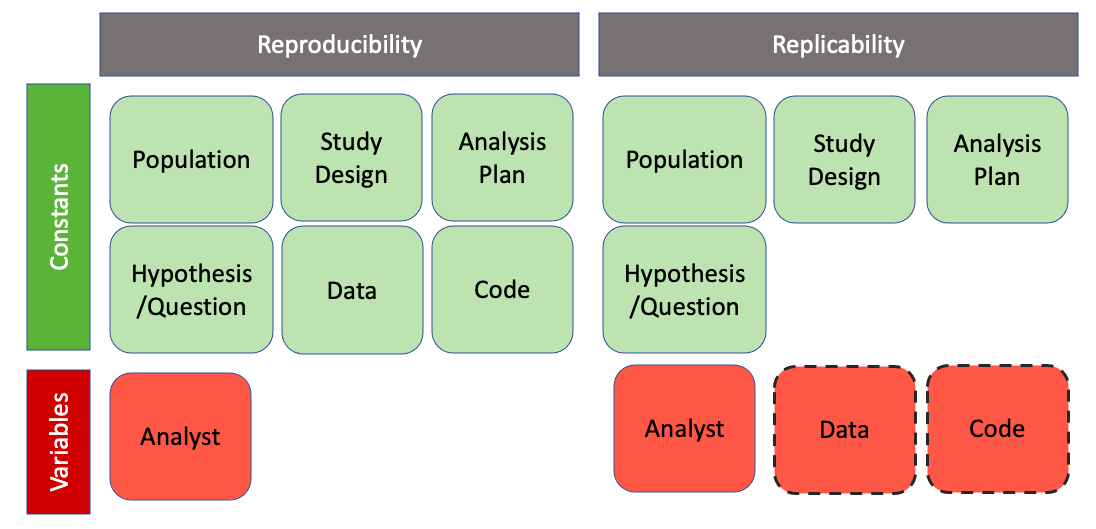
\includegraphics[width=1\linewidth]{figure/versus} 

}

\caption{Reproducibility vs. Replicability}\label{fig:unnamed-chunk-3}
\end{figure}
Reproducibility and replicability are both necessary to the advancement
of scientific research, but they vary significantly in terms of their
difficulty to achieve. Reproducibility, in theory, is somewhat simple to
attain in data analyses--because code is inherently non-random
(excepting applications involving random number generation) and data
remain consistent, variability is highly restricted. The achievement of
replicability, on the other hand, is a much more complex challenge,
involving significantly more variablility and requiring high quality
data, effective study design, and incredibly robust hypotheses.

\section{The Reproducibility Crisis}\label{the-reproducibility-crisis}

Despite the relative simplicity of achieving reproducibility, a
significant proportion of the work produced in the scientific community
fails to meet reproducibility standards. 52\% of respondents in a 2016
Nature survey believed that science was going through a ``crisis'' of
reproducibility. Additionally, the vast majority of researchers across
all fields studied reported having been unable to reproduce another
researcher's results, while approximately half reported having been
unable to reproduce their own (Baker (2016)). Other studies paint an
even bleaker picture: a 2015 study found that over 50\% of studies
psychology failed reproducibility tests and research from 2012 found
that figure closer to 90\% in the field of cancer biology (Baker (2015),
Begley \& Ellis (2012)).

In the past several years, this ``crisis'' of reproducibility has risen
toward the forefront of scientific discussion. Without reproducibility,
the scientific community cannot properly verify study results.This makes
it difficult to identify which information should be believed and which
should not and increases the likelihood that studies sharing misleading
information will be dispersed. The rise of data-driven technologies,
alongside our newly founded ability to instantly share knowledge
worldwide, has made reproducibility increasingly critical to the
advancement of scientific understanding, necessitating the development
of solutions for addressing the issue.

Academics have recognized this, and publications on the topic appear to
have increased siginficantly in the last several years (Eisner (2018);
Fidler \& Wilcox (2018); Gosselin (2020); McArthur (2019); Wallach,
Boyack, \& Ioannidis (2018)).

\section{The Components of Reproducible
Research}\label{the-components-of-reproducible-research}

In order to see why there is an issue with reproducibility and gain a
sense of how to solve it, it is important to first understand the
components of reproducibility. Essentially, to answer, ``What parts does
researcher need to include, or what steps do they need to take, to be
able to declare their work reproducible?''

Publications attempting to answer this can be found in all areas of
scientific research. However, as Goodman et al. (2016) argue, the
language and conceptual framework used to describe research
reproducibility varies significantly across the sciences, and there are
no clear standards on reproducibility agreed upon by the scientific
community as a whole.

At a minimum, according to Goodman et al. (2016), achieving
reproducibility requires the sharing of data (raw or processed),
relevant metadata, code, and related software. However, according to
other authors, the full achievement of reproducibility may require
additional components.

Kitzes, Turek, \& Deniz (2017) present a collection of case studies on
reproducibility practices from across the data-intensive sciences,
illustrating a variety of recommendations and techniques for achieving
reproducibility. Although their work does not come to a consensus on the
exact standards of reproducibility that should be followed, several
common trends and principles emerge from their case studies that extend
beyond the minimum recommendations of Goodman et al. (2016):
\begin{enumerate}
\def\labelenumi{\arabic{enumi})}
\tightlist
\item
  use clear separation, labeling, and documentation in provided code,
\item
  automate processes when possible, and
\item
  design the data analysis workflow as a sequence of small steps glued
  together, with outputs from one step serving as inputs into the next.
  This is a common suggestion within the computing community,
  originating as part of the Unix philosophy (Gancarz (2003)).
\end{enumerate}
Cooper et al. (2017) focus on data analysis completed in \texttt{R} and
identify a similar list of important reproducibility components,
reinforcing the need for clearly labeled, well-documented, and
well-separated files. In addition, they recommend publishing a list of
software dependencies and using version control to track project changes
over time.

Broman (2019) reiterates the need for clear naming and file separation
while sharing several additional suggestions: keep the project contained
in one directory, use relative paths when accessing the file system, and
include a \texttt{README} file describing the project.

The reproducibility recommendations from R OpenSci, a non-profit
initiative founded in 2011 to make scientific data retrieval
reproducible, share similar principles to those discussed previously.
They focus on a need for a well-developed file system, with no
extraneous files and clear labeling. They also reiterate the need to
note dependencies and use automation when possible, while making clear a
suggestion not present in the previously-discussed literature: the need
to use seeds, which allow for the saving and restoring of the random
number generator state, when running code involving randomness (Martinez
et al. (2018)).

Although these recommendations differ from one another, when considered
in combination they provide a well-rounded picture of the components
important to research reproducibility across the scientific community:
\begin{enumerate}
\def\labelenumi{\arabic{enumi}.}
\tightlist
\item
  The basic project components are made accessible to the public:
\end{enumerate}
\begin{itemize}
\tightlist
\item
  Data (raw and/or processed)
\item
  Metadata
\item
  Code
\item
  Related Software
\end{itemize}
\begin{enumerate}
\def\labelenumi{\arabic{enumi}.}
\setcounter{enumi}{1}
\tightlist
\item
  The file structure of project is well-organized:
\end{enumerate}
\begin{itemize}
\tightlist
\item
  Separate folders for different file types.
\item
  No extraneous files.
\item
  Minimal clutter.
\end{itemize}
\begin{enumerate}
\def\labelenumi{\arabic{enumi}.}
\setcounter{enumi}{2}
\tightlist
\item
  The project is documented well:
\end{enumerate}
\begin{itemize}
\tightlist
\item
  Files are clearly named, preferably in a way where the order in which
  they should be run is clear.
\item
  A README is present.
\item
  Code contains comments.
\item
  Software dependencies are noted.
\end{itemize}
\begin{enumerate}
\def\labelenumi{\arabic{enumi}.}
\setcounter{enumi}{3}
\tightlist
\item
  File paths used in code are not system- or user-dependent:
\end{enumerate}
\begin{itemize}
\tightlist
\item
  No absolute paths.
\item
  No paths leading to locations outside of a project's directory.
\item
  Only relative paths, pointing to locations within a project's
  directory, are permitted.
\end{itemize}
\begin{enumerate}
\def\labelenumi{\arabic{enumi}.}
\setcounter{enumi}{4}
\tightlist
\item
  Randomness is accounted for:
\end{enumerate}
\begin{itemize}
\tightlist
\item
  If randomness is used in code, a seed must also be set.
\end{itemize}
\begin{enumerate}
\def\labelenumi{\arabic{enumi}.}
\setcounter{enumi}{5}
\tightlist
\item
  Code is readable and consistently styled:
\end{enumerate}
\begin{itemize}
\tightlist
\item
  Though not mentioned in the sources described previously, it is also
  important that code be written in a coherent style. This is because
  code that conforms to a style guide or is written in a consistent
  dialect is easier to read, simplifying the process of following a
  researcher's work from beginning to end (Hermans \& Aldewereld
  (2017)).
\end{itemize}
\section{Current Attempts to Address Reproducibility in Scientific
Publishing}\label{current-attempts-to-address-reproducibility-in-scientific-publishing}

In an attempt to increase reproducibility, leaders from academic
journals around the world have taken steps to create new standards and
requirements for submitted articles. These standards attempt to address
the components of reproducibility listed previously, requesting that
authors provide certain materials necessary for reproducibing their work
when they submit an article. However, these standards are highly
inconsistent, varying significantly both across and within disciplines,
and many only cover one or two of the six primary components, if any at
all.

To illustrate this point, we will consider several case studies from
journals publishing research on a variety of scientific fields.

\subsection{Case Studies Across The
Sciences}\label{case-studies-across-the-sciences}

The journal whose requirements appear to align most closely with those
components defined previously in Section 3 is the \emph{American Journal
of Political Science} (AJPS). In 2012, the AJPS became the first
political science journal to require authors to make their data openly
accessible online, and the publication has instituted stricter
requirements since. AJPS now requires that authors submit the following
alongside their papers (American Journal of Political Science (2016)).
\begin{itemize}
\tightlist
\item
  The dataset analyzed in the paper and information about its source. If
  the dataset has been processed, instructions for manipulating the raw
  data to achieve the final data must also be shared.
\item
  Detailed, clear code necessary for reproducing all of the tables and
  figures in the paper.
\item
  Documentation, including a README and codebook.
\item
  Information about the software used to conduct the analysis, including
  the specific versions and packages used.
\end{itemize}
These standards are quite thorough and contain mandates for the
inclusion of the vast majority of components necessary for complete
reproducibility. Most journals, however, do not come close to meeting
such high standards in their reproducibility statements.

For example, in the biomedical sciences, a group of editors
reproesenting over 30 major journals met in 2014 to address
reproducibility in their field, coming to a consensus on a set of
principles they wanted to uphold (National Institutes of Health (2014)).
Listed below are those relating specifically to the use of data and
statistical methods:
\begin{enumerate}
\def\labelenumi{\arabic{enumi})}
\item
  Journals in the biomedical sciences should have a mechanism to check
  the statistical accuracy of submissions.
\item
  Journals should have no (or generous) limit on methods section length.
\item
  Journals should use a checklist to ensure the reporting of key
  information, including:
\end{enumerate}
\begin{itemize}
\tightlist
\item
  The article meets nomenclature/reporting standards of the biomedical
  field.
\item
  Investigators report how often each experiment was performed and
  whether results were substantiated by repetition under a range of
  conditions.
\item
  Statistics must be fully reported in the paper (including test used,
  value of N, definition of center, dispersion and precision measures).
\item
  Authors must state whether samples were randomized and how.
\item
  Authors must state whether the experiment was blinded.
\item
  Authors must clearly state the criteria used for exclusion of any data
  or subjects and must include all results, even those that do not
  support the main findings.
\end{itemize}
\begin{enumerate}
\def\labelenumi{\arabic{enumi})}
\setcounter{enumi}{3}
\item
  All datasets used in analysis must be made available on request and
  should be hosted on public repositories when possible. If not
  possible, data values should be presented in the paper or
  supplementary information.
\item
  Software sharing should be encouraged. At the minimum, authors should
  provide a statement describing if software is available and how to
  obtain it.
\end{enumerate}
Even though these principles seem well-developed on the surface, they
fail to meet even the basic requirements defined by Goodman et al.
(2016) previously. Several of the principles are purely recommendations;
there is no requirement that code be shared, nor metadata. Additionally,
software requirements are quite loose, requiring no information about
dependencies or software version.

We see a similar issue even in journals designed specifically for the
purpose of improving scientific reproducibility. \emph{Experimental
Results}, a publication created by Cambridge University Press to address
some of the reproducibility and open access issues in academia, also
falls short of meeting high standards. The journal, which showcases
articles from a variety of scientific decisions disciplines, states in
their transparency and openness policy:
\begin{quote}
Whenever possible authors should make evidence and resources that
underpin published findings, such as data, code, and other materials,
available to readers without undue barriers to access.
\end{quote}
The inclusion of code and data are only recommended and no definition of
what ``other materials'' may mean is provided. No components of
reproducibility extending beyond those required at a minimum are even
considered (Cambridge University Press (2020)).

The \emph{American Economic Review}, the first of the top economics
journals to require the inclusion of data alongside publications, has
stronger guidelines than several of those mentioned previously, though
not as strong as the \emph{American Journal of Political Science}. Their
Data and Code Availability Policy states the following (American
Economic Association (2020)):
\begin{quote}
It is the policy of the American Economic Association to publish papers
only if the data and code used in the analysis are clearly and precisely
documented, and access to the data and code is clearly and precisely
documented and is non-exclusive to the authors.
\end{quote}
These requirements are quite strict, prohibiting exceptions for papers
using data or code not available to the public in the way that many
other journals claiming to promote reproducibility do.

\subsection{Case Studies In The Statistical And Data
Sciences}\label{case-studies-in-the-statistical-and-data-sciences}

When considering reproducibility policy, the field of Statistical and
Data Sciences performs relatively well. The majority of highly ranked
journals in the field contain statements on reproducibility. Some of
these are quite robust, surpassing the requirements of many of the other
journals discussed previously, while others are lacking.

The \emph{Journal of the American Statistical Association} stands out as
having relatively robust requirements. The publication's guideliens
require that data be made publicly available at the time of publication
except for reasons of security or confidentiality. It is strongly
recommended that code be deposited in open repositories. If data is used
in a process form, the provided code should include the necessary
cleaning/preparation steps. Data must be in an easily understood form
and a data dictionary should be included. Code should also be in a form
that can be used and understood by others, including consistent and
readable syntax and comments. Workflows involving more than one script
should also contain a master script, Makefile, or other mechanism that
makes it clear what each component does, in what order to run them, and
what the inputs and outputs to each area (American Statistical
Association (2020)).

The \emph{Journal of Statistical Software} also has strong guidelines,
though less thorough. Authors must provide \emph{commented} source code
for their software; all figures, tables, and output must be exactly
reproducible on at least one platform, and random number generation must
be controlled; and replication materials (typically in the form of a
script) must be provided (Journal of Statistical Software (2020)).

The expectations of the \emph{Journal of Computational and Graphical
Statistics} are notably weaker, requiring only that authors ``submit
code and datasets as online supplements to the manuscript,'' with
exceptions for security or confidentiality, but providing no further
detail (Journal of Computational and Graphical Statistics (2020)). The
\emph{R Journal} has the same requirements, but with no exceptions on
the data provision policy, stating that authors should ``not use such
datasets as examples'' (R Journal Editors (2020)).

Perhaps the weakest reproducibility policies come from \emph{The
American Statistician} and the \emph{Annals of Statistics}. The former
appears to have no requirements, stating only that it ``strongly
encourages authors to submit datasets, code, other programs, and/or
appendices that are directly relevant to their submitted articles,''
while the latter appears to have no statement on reproducibility at all
(The American Statistician (2020)).
\begin{figure}

{\centering 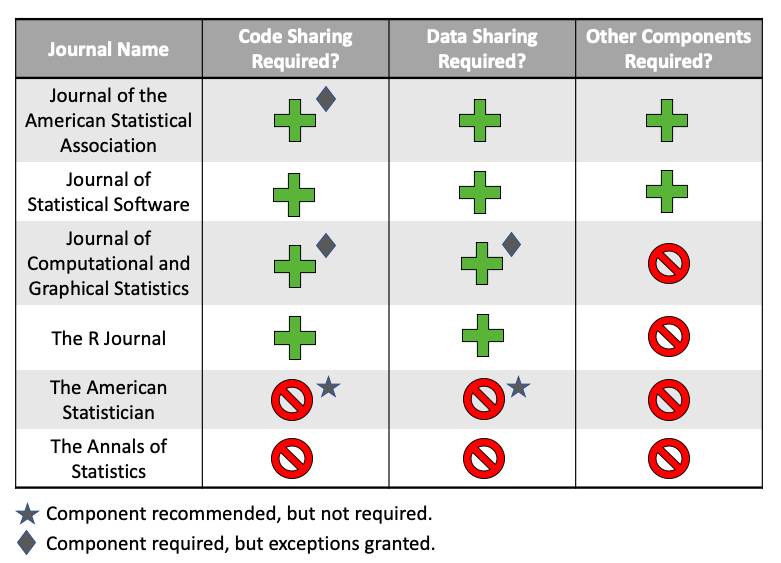
\includegraphics[width=1\linewidth]{figure/stats-journals} 

}

\caption{Reprodubility Policies of Top Statistical and Data Sciences Journals}\label{fig:unnamed-chunk-4}
\end{figure}
\subsection{The Bigger Picture}\label{the-bigger-picture}

The journals mentioned here are just some of the many academic
publishers with reproducibility policies. While they provide a sense of
the specific wording and requirements of some policies, they do not
necessarily serve as a representative sample of all academic publishing.
It is important to also consider the bigger picture, exploring the state
of reproducibility policy in academic publishing as a whole.

Given the scale of the academic publishing network and the sheer number
of journals around the world, this is not necessarily an easy task.

In order to simplify this process, academics at the Center for Open
Science (COS) attempted to create a metric, called the TOP Factor. The
TOP Factor reports the steps that a journal is taking to implement open
science practices. It has been calculated for a wide variety of
journals, though the COS is still far from scoring all of the
publications that are currently available.

The TOP Factor is calculated as follows. Publications are scored on a
variety of categories associated with open science and reproducibility.
For each category, they receive a score between 0 (poor) and 3
(excellent) based on the degree to which they emphasize each category in
their submission/publication policies. A journal's final score, which
can range from 0 to 30, is the sum of the individual scores in each of
the categories.
\begin{center}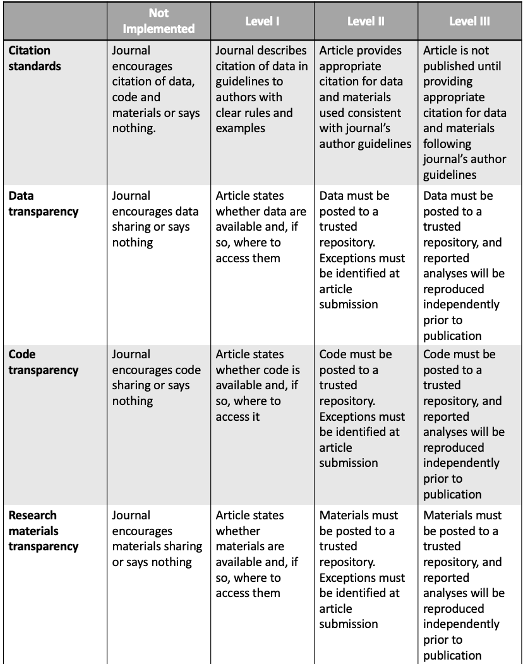
\includegraphics[width=1\linewidth]{figure/top-1} \end{center}
\begin{figure}

{\centering 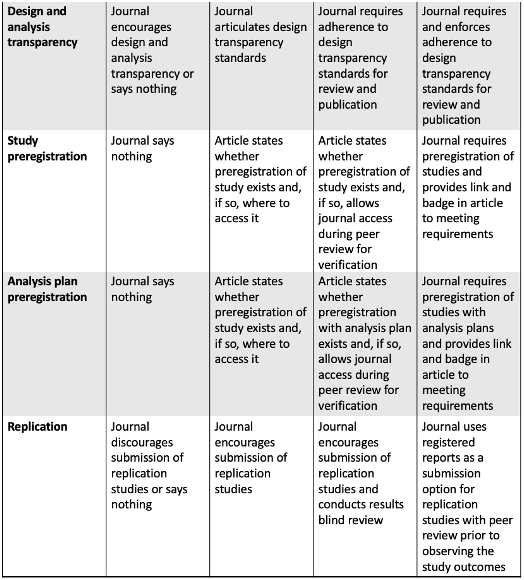
\includegraphics[width=1\linewidth]{figure/top-2} 

}

\caption{The TOP Factor Rubric}\label{fig:top-factor2}
\end{figure}
When looking at the overall distribution of TOP Factor scores, we see a
relatively grim picture: Around 50\% of journals score as low as 0-5
overall, while only just over 5\% score more than 15, just half of the
maximum possible score. Over 40 journals failed to score a single point
(Woolston (2020)).

Although it is clear that some journals have relatively strong
reproducibility and openness policies, that is clearly not the norm. And
many that do appear to have policies lacking in robustness, including
exceptions for data privacy and security concerns or phrasing guidelines
as recommendations rather than reqquirements. The field of data science
stands out among the rest, with the majority of top journals having
relatively robust policies.

\subsection{Assessing the Success of Academic Reproducibility
Policies}\label{assessing-the-success-of-academic-reproducibility-policies}

We have seen that, although not necessarily the standard, some journals
across the sciences have enacted reproducibility policies. The simple
implementation of a policy, however, does not ensure that its goals will
be achieved. Reproducibility can only be addressed when both authors
\emph{and} journal reviewers actively implement publishing standards in
practice. Without participation and dedication from all involved,
reproducibility guidelines serve more as a theoretical goal than a
practical achievement.

It is important to ask, then, whether academic reproducibility standards
\emph{actually} result in a greater number of reproducible publications.

Let us consider the case of the journal \emph{Science}. \emph{Science}
instituted a reproducibility policy in 2011 and has maintained it ever
since. In its original form, their policy stated the following:
\begin{quote}
All data necessary to understand, assess, and extend the conclusions of
the manuscript must be available to any reader of Science. All computer
codes involved in the creation or analysis of data must also be
available to any reader of Science. After publication, all reasonable
requests for data and materials must be fulfilled. Any restrictions on
the availability of data, codes, or materials\ldots{}must be disclosed
to the editors upon submission\ldots{}
\end{quote}
This policy is similar to many of the others considered previously,
requiring the publishing of code and data with exceptions permitted when
necessary.

Stodden, Seiler, \& Ma (2018a) tested the efficacy of this policy in
practice, emailing corresponding authors of 204 articles published in
the year after \emph{Science} first implmented its policy to request the
data and code associated with their articles. The researchers only
received (at least some of) the requested material from 36\% of authors.
This low rates were due to several factors:
\begin{itemize}
\tightlist
\item
  26\% of authors did not respond to email contact.
\item
  11\% of authors were unwilling to provide the data or code without
  further information regarding the researchers' intentions.
\item
  11\% asked the researchers to contact someone else and that person did
  not respond.
\item
  7\% refused to share data and/or code.
\item
  3\% directed the researchers back to their paper's supplmental
  information section.
\item
  3\% of authors made a promise to follow up and then did not follow
  through.
\item
  3\% of emails bounced.
\item
  2\% gave reasons why they could not share for ethical reasons, size
  limitations, or some other reason.
\end{itemize}
Of the 56 papers they deemed likely reproducible, the authors randomly
selected 22 and were able to replicate the results for all but 1, which
failed due to its reliance on software that was no longer available.

Hardwicke et al. (2018) conducted a study on the journal
\emph{Cognition}, where researchers compared the reproducibility of
published work both before and after the journal instituted an open data
policy, which required that authors make relevant research data publicly
available prior to publication of an article.

The researchers found a considerable increase in the proportion of data
available statements (in constrast to `data not available' statements,
which could be present due to privacy or security concerns) since the
implementation of the policy. Pre-open data policy, only 25\% of
articles had data available, while that number was a much higher 78\%
after the policy was put in place.

While the institution of an open data policy appears to have been
associated with a significant increase in the percentage of studies with
data available, further research indicates that the policy was perhaps
not as effective as intended. Many of the datasets were usable in
theory, but not in practice. Only 62\% of the articles with data
available statements had truly reusable datasets--in this case, meaning
that the data were accessible, complete, and understandable. Though this
is an increase from the pre-policy period, which saw 49\% of articles
with data availability statements as reusable in practice, it is still
far from ideal.

Combining these two data points indicates that \emph{less than half} of
articles published after the open data policy was instituted actually
contained truly usable data.

In this small sample of cases, we see that purely having a
reproducibility statement does not necessarily mean that all, or even a
majority, of published work will truly be reproducible.

\section{Limitations on Achieving Reproducibility in Scientific
Publishing}\label{limitations-on-achieving-reproducibility-in-scientific-publishing}

There are several reasons for this apparent divide between journal
reproducibility standards and the true proportion of submitted articles
that are truly reproducible. Some of these are challenges faced by the
article authors, while others are faced by the journal editors.

\subsection{Challenges for Authors}\label{challenges-for-authors}

Stodden, Seiler, \& Ma (2018b) conducted a survey asking over 7,700
researchers about one of the key characteristics of reproducibility --
open data -- and gathered information about the reasons why authors
found difficulties in making their data available to the public

The main challenges listed by respondents were as follows:
\begin{itemize}
\tightlist
\item
  46\% identified ``Organizing data in a presentable and useful way'' to
  be difficult.
\item
  37\% had been ``Unsure about copyright and licensing.''
\item
  33\% had problems with ``Not knowing which repository to use.''
\item
  26\% cited a ``Lack of time to deposit data.''
\item
  19\% found the ``Costs of sharing data'' to be high.
\end{itemize}
The relative frequency of these issues varied across several
characteristics, including author seniority, subject area, and
geographical location, though authors in all categories faced some
issues.

Beyond technical challenges, other reasons may lead authors to not place
their focus on reproducibility. For example, some researchers might fear
damage to their reputation if a reproduction attempt fails after they
have provided the necessary materials (Lupia \& Elman (2014)).

Given the relatively high frequency of concern over achieving
reproducibility, it follows that researchers will not make the necessary
effort to do so if journal guidelines provide a way out. Policies that
\emph{recommend} the inclusion of data or that allow exceptions to open
data for certain reasons are likely to be associated with a lower
proportion of reproducible articles than those that make open data
mandatory.

\subsection{Challenges for Journals}\label{challenges-for-journals}

In addition to the challenges faced on the part of the authors, journal
reviewers face their own difficulties in ensuring reproducibility.

In order to make sure that all submitted articles comply with
reproducibility guidelines, reviewers must go through them one by one
and reproduce all of the results by hand using the provided materials.

This is an incredibly intensive process, as we will see in the example
of the \emph{American Journal for Political Science} (AJPS), whose
reproducibility policy was discussed prevously in Chapter 1.4.1.

Jacoby, Lafferty-Hess, \& Christian (2017) describe the AJPS process in
detail:

Acceptance of an article for publication in the AJPS is contingent on
successful reproducibility of any empirical analyses reported in the
article.

After an article is submitted, staff from a third party vendor hired by
AJPS go through the provided materials to ensure that they can be
preserved, understood, and used by others. They then run all of the
analyses in the article using the code, instructions, and data provided
by the authors and compare their results to the submitted articles.
Authors are then given an opportunity to resolve any issues that come
up. This process is repeated until reproducibility is ensured.

Although providing a significant benefit to the scientific community,
this thorough process is associated with high costs.

The verification process slows down the journal review process
significantly, adding a median 53 days to the publication workflow, as
many submitted articles require one or more rounds of resubmission (the
average number of resubmissions is 1.7). It is also quite labor
intensive, taking an average of 8 person-hours per manuscript to
reproduce the analyses and prepare the materials for public release and
adding significant monetary cost to AJPS.

Journals are often reluctant to take on such an intensive task due to
the drastically increased burden it places on reviewers and on the
publication's financial resources. This is particularly true given that
the number of submitted articles per year has been increasing over time
(Leopold (2015)). Every additional submission increases the burden of
achieving reproducibility, and with a large enough volume, the challenge
can quickly become seemingly impossible to manage reasonably.

As a result, journals often encourage reviewers to consider authors'
compliance with data sharing policies, but do not formally require that
they ensure it as a criterion for acceptance (Hrynaszkiewicz (2020)).

\section{Attempts to Address These
Limitations}\label{attempts-to-address-these-limitations}

The previous discussion makes clear that, although reproducibility is
critically important to scientific progress and academic journals are
taking steps to encourage it, the scientific community is far from
achieving the desired level of widespread reproducibility. In large
part, this appears due to the challenge and complexity of actually
achieving reproducibility. Those attempting to improve the
reproducibility of work can face issues with concerns over legality of
sharing data, large commitments of time or money, challenges finding a
good repository, and organizing all of the many components of their work
in an understandable way, among other things.

Additionally, science faces the additional challenge that many
publishers do not emphasize reproducibility at all, providing many
opportunities for all authors except those personally dedicated to
producing reproducible work to leave reproducibility by the wayside.
Many journals have no reproducibility requirements, and those that do
often do not take the necessary steps to ensure that they are actually
met.

These issues, however, are not impossible to overcome. Proponents of
reproducibility have taken action to help address them, both through
education on reproducibility and through software that helps simplify
the process of achieving it.

\subsection{Through Education}\label{through-education}

One way to address the reproducibility crisis is to educate data
analysts on the topic so that they are aware of both the concept of
reproducibility and how to achieve it in their own work. A natural place
to focus this education is early on in the data science training
pipeline as part of introductory or early-intermediate courses in
undergraduate and graduate data science porgrams (Horton, Baumer, \&
Wickham (2014)). This sort of educational integration has a variety of
benefits:
\begin{itemize}
\item
  Bringing reproducibility into the discussion early on gives students
  the tools to add knowledge to their field in the best way possible
  before they actually conduct any substantive analysis on their own
  (Janz (2016)). This produces many long run benefits, helping lessen
  the burden on promoting reproducibility placed on journals and
  increasing the number (and percentage) of researchers doing and
  promoting reproducible work.
\item
  If covered in detail as part of the data science curriculum,
  reproducibility will eventually come easily to students. If learned
  independently, without effective tools, reproducibility can
  challenging and even disheartening to try to understand and succeed
  at. Practicing in the classroom gives students the ability to fail
  without damaging their reputation, giving a great opportunity to truly
  learn and understand the concepts so that they feel capable of
  handling them when they begin their own research.
\item
  The application of grading to the topic provides an incentive for
  students to pay attention, learn, and absorb the information. This
  same incentive does not exist when researchers attempt to learn about
  reproducibility independently. In that situation, internal motivation,
  which may be weak in some individuals, is the only factor present to
  help promote success.
\end{itemize}
Several educators, primarily at the graduate level, have realized the
opportunity and taken steps to introduce reproducibility into their
courses. According to Janz (2016), the primary way of achieving this
integration is through the assignment of ``replication studies'' in
standard methods choices. In these assignments, students are given a
published study and its supporting materials and asked to reproduce the
results. The most famous course of this kind is Government 2001, taught
by Gary King at Harvard University. In King's course, students team up
in small groups to reproduce a previous study. To help ensure that their
workflow is reproducible, students are required to hand over their data
and code to another student team who then tries to reproduce their work
once again.

In Thomas M. Carsey's intermediate statistics course at the University
of North Carolina at Chapel Hill, students must reproduce the findings
of a study by re-collecting the data from the original sources, then
must extend the study by building on the analysis.

Christopher Fariss of Penn State University asks his students to
replicate a research paper published in the last five years, noting that
students must describe the article and the ease in which the results
replicate.

The University of California at Berkeley has a similar course to Gary
King's Harvard course, where students each take a different piece of an
existing study to work on reproducing and have to ensure that their
piece fits with the piece of the next student (Hillenbrand (2014)).

At the undergraduate level, rather than assign replication studies the
way many graduate schools tend to do, Smith College and Duke University
have both integrated reproducibility into their introductory courses
through the requirement that assignments be completed in the
\texttt{RMarkdown} code + narration format (B. Baumer, Cetinkaya-Rundel,
Bray, Loi, \& Horton (2014)).

Another way to provide education on reproducibility is through the
creation of workshops that focus solely on the topic, rather than
through integration as just one part of a class (@Janz (2016)).

For example, the University of Cambridge conducts a Replication
Workshop, where graduate students are asked replicate a paper in their
field over eight weekly sessions. When students encounter challenges,
such as authors not responding to queries for data or steps of the
analysis being poorly defined and explained, they gain a first hand
understanding of the consequences of poor transparency.

Workshops such as these are typically optional and not included as part
of the primary curriculum, however, so while they may cover the topic of
reproducibility in more detail than traditional courses, they often
reach fewer students.

In spite of all of the advantages that these educational tools provide,
``reproducibility training and assessment in data science education is
largely neglected, especially among undergraduates and Master's students
in professional schools\ldots{}, probably because the students are
usually considered to be non-research oriented'' (Yu \& Hu (2019)).
While some examples of reproducibility education exist, they are
certainly not commonplace. However, given the increased discussion and
emphasis on reproducibility in academia over the past several years, it
is likely that this will change, particularly if methods are provided to
educators to make the integration of reproducibility into their courses
simple and relatively unburdensome.

\subsection{Through Software}\label{through-software}

Several researchers and members of the Statistical and Data Sciences
community have taken action to develop software focused on
reproducibility which removes some of the load on data analysts by
automating reproducibility processes and checking whether certain
components are achieved.

Much of this software has been written for users of the coding and data
analysis language \texttt{R}. \texttt{R} is very popular in the data
science community due to its open-source nature, accessibility,
extensive developer and user base, and statsitical analysis-specific
features.

Some of the existing software solutions are listed below:

\texttt{rrtools} (Marwick (2019)) addresses many of the issues discussed
in Marwick, Boettiger, \& Mullen (2018) by creating a basic reproducible
structure based on the \texttt{R} package format for a data analysis
project. In addition, it allows for isolation of the computer
environment using \texttt{Docker}, provides a method to capture
information about the versions of packages used in a project, contains
tools for generating a README file, and provides an option for users to
write tests to check that their functions operate as intended.

The \texttt{orderly} (FitzJohn et al. (2020)) package also focuses on
file structure, requiring the user to declare a desired project
structure (typically a step-by-step structure, where outputs from one
step are inputs into the next) at the beginning and then creating the
files necessary to achieve that structure. Its principal aim is to
automate many of the basic steps involved in writing analyses, making it
simple to:
\begin{enumerate}
\def\labelenumi{\arabic{enumi})}
\tightlist
\item
  Track all inputs into an analysis.
\item
  Store multiple versions of an analysis where it is repeated.
\item
  Track outputs of an analysis.
\item
  Create analyses that depend on the outputs of previous analyses.
\end{enumerate}
When projects have a variety of components, \texttt{orderly} makes it
easy to see inputs and outputs change with each re-run.

\texttt{workflowr}'s (Blischak, Carbonetto, \& Stephens (2019))
functionality is based around version control and making code easily
available online. It works to generate a website containing
time-stamped, versioned, and documented results. In addition, it manages
the session and package information of each analysis and controls random
number generation.

\texttt{checkers} (Ross, DeCicco, \& Randhawa (2018)) allows you to
create custom checks that examine different aspects of reproducibility.
It also contains some pre-built checks, such as seeing if users
reference packages that are less preferred to other similar ones and
ensuring that the project is under version control. \texttt{renv} (Ushey
\& RStudio (2020)) (formerly \texttt{packrat}) helps to make projects
more isolated, portable, and reproducible. It gives every project its
own private package library, makes it easy to install the packages the
project depends on if it is moved to another computer.

\texttt{drake} (OpenSci (2020)) analyzes workflows, skips steps where
results are up to date, utilizes optimized computing to complete the
rest of the steps, and provides evidence that results match the
underlying code and data.

Lastly, the \texttt{reproducible} (McIntire \& Chubaty (2020)) package
focuses on the concept of caching: saving information so that projects
can be run faster each time they are re-completed from the start.
\begin{figure}

{\centering 
\includegraphics[width=0.5\linewidth]{figure/packages} 

}

\caption{Popular Reproducibility Packages in R}\label{fig:unnamed-chunk-5}
\end{figure}
There have also been several \texttt{Continuous\ integration} tools
developed outside of R which can be used by those coding in almost any
language. These provide more general approaches to automated checking,
which can enhance reproducibility with minimal code.

For example, \texttt{wercker}---a command line tool that leverages
Docker---enables users to test whether their projects will successfully
compile when run on a variety of operating systems without access to the
user's local hard drive (Oracle Corporation (2019)).

\texttt{GitHub\ Actions} is integrated into GitHub and can be configured
to do similar checks on projects hosted in repositories.

\texttt{Travis\ CI} and \texttt{Circle\ CI} are popular continuous
integration tools that can also be used to check \texttt{R} code.
\begin{figure}

{\centering 
\includegraphics[width=0.8\linewidth]{figure/ci-tools} 

}

\caption{Popular Continuous Integration Tools}\label{fig:unnamed-chunk-6}
\end{figure}
\section{Understanding The Gaps In Existing Reproducibility
Solutions}\label{understanding-the-gaps-in-existing-reproducibility-solutions}

Although the current state of reproducibility in academia is quite poor,
it is not an impossible challenge to overcome. The relative simplicity
of addressing reproducibility, particularly when compared with
replicability, makes it an ideal candidate for solution-building.
Although significant progress on addressing reproducibility on a
widespread scale is a long-term challenge, impactful forward
progress--if on a smaller scale--can be achieved in the short-term.

As we have seen, software developers, data scientists, and educators
around the world have realized this potential, taking steps to help
address the current crisis of reproducibility. Journals have put in
place guidelines for authors, statisticians have developed \texttt{R}
packages that help structure projects in a reproducible format, and
educators have begun integrate reproducibility exercises into their
courses.

We have already explored the issues with journal policies, both for
authors and reviewers, in-depth. Educational and software-based
strategies attempt to address these policy issues by spreading ideas of
reproducibility to more people and simplifying the process of achieving
it, therefore resulting (in theory) in an improvement in the
reproducibility of published scientific articles.

However, the reality is not quite so rosy. Many current educational and
software-based solutions face their own challenges that limit them from
achieving the desired outcome. In this section, we will consider these
issues.

\subsection{In Education}\label{in-education}

The two primary concerns about the integration of reproducibility in
data science curricula revolve around time and difficulty.

As noted previously, the primary mode of teaching reproducibility is
through the assignment of replication studies where students must take
an existing study and go through the process of reproducing it
themselves, including contacting the author for all necessary materials,
rerunning code and analysis, and problem-solving when issues almost
certainly come up.

In addition to the time required for the professor to collect all of the
studies that students will be working on, the inclusion of such an
assignment places a significant burden on educators by taking up time
where they could be teaching other important material. Replication
studies, if done correctly, can take weeks for students to successfully
complete. The choice to give such assignments is therefore associated
with a significant opportunity cost which many professors are unwilling
to take.

Additionally, both replication studies assigned in class and replication
workshops outside of normal coursework require a working knowledge of
how to successfully complete and understand research. This makes them
inaccessible to individuals who are still in their undergraduate career
and may not yet have had an opportunity to conduct research or those who
are studying in non-research-focused technical programs.

In order to reach the widest variety of students possible, it is
necessary to develop a new method of teaching reproducibility that is
neither time consuming nor dependent on a prior understanding of the
research process.

\subsection{In Software}\label{in-software}

Previously, we considered several different types of software solutions:
packages designed for users of \texttt{R} and continuous integration
programs that can be used alongside a variety of coding languages.
Although these solutions have their advantages, they also have
significant drawbacks in terms of their ability to address
reproducibility on a widespread scale.

Many of the packages designed for \texttt{R} are incredibly narrow in
scope, with each effectively addressing a small component of
reproducibility: file structure, modularization of code, version
control, etc. They often succeed in their area of focus, but at the cost
of accessibility to a wider audience. Their functions are often quite
complex to use, and many steps must be completed to achieve the required
reproducibility goal. This cumbersome nature means that most
reproducibility packages currently available are not easily accessible
to users with minimal \texttt{R} experience, nor particularly useful to
those looking for quick and easy reproducibility checks. The significant
learning curve associated with them can also detract potential users who
may be interested in reproducibility but not willing to dedicate an
extensive amount of time to understanding the intricacies of software
operation.

Due to their generalized design, Continuous Integration tools do not
face the same issues with narrowness or complexity that \texttt{R}
packages struggle with. However, this generalizability provides its own
additional challenge. Since Continuous Integration tools are designed to
be accessible to a wide variety of users with different coding
preferences, they are not particularly customizable and lack the ability
to address features specific to certain programming languages.

Neither of these different software solutions appear to adequately
address the challenge of reproducibility.

\subsection{What We Need Moving
Forward}\label{what-we-need-moving-forward}

While a variety of attempts to address reproducibility have been made,
they all face their own set of challenges. Most focus on only one area
of reproducibility, are too time consuming and burdensome to attempt, or
require an extensive amount of background knowledge.

In order to truly improve scientific reproducibility, a better solution
is needed. The optimal solution should combine the positive aspects of
the previously discussed educational and software methods, while
remaining simple and easy to use. It should also have a variety of
potential applications---journal reviewers should benefit from it, as
should authors, as should educators and students and even those outside
of academia.

The full list of necessary features for an effective reproducibility
tool are provided below:
\begin{enumerate}
\def\labelenumi{\arabic{enumi})}
\tightlist
\item
  Be simple, with a small library of functions/tools that are
  straightforward to use.
\item
  Be accessible to a variety of users, with a relatively small learning
  curve.
\item
  Be able to address a wide variety of aspects of reproducibility,
  rather than just one or two key issues.
\item
  Have features specific to a particular coding language that can
  address that language's unique challenges.
\item
  Be customizable, allowing users to choose for themselves which aspects
  of reproducibility they want to focus on.
\item
  Be educational, teaching those that use it about why their projects
  are not reproducible and how to correct that in the future.
\item
  Be applicable to a wide variety of domains and users.
\end{enumerate}
While this seems like a lot to ask, such a task is not impossible. In
the next chapter, we will consider one potential solution:
\texttt{fertile}, an R package focused on reproducibility that I have
worked to develop.

\chapter{\texorpdfstring{\texttt{fertile}: My Contribution To Addressing
Reproducibility}{fertile: My Contribution To Addressing Reproducibility}}\label{my-solution}

\section{\texorpdfstring{\texttt{fertile}, An R Package Creating Optimal
Conditions For
Reproducibility}{fertile, An R Package Creating Optimal Conditions For Reproducibility}}\label{fertile-an-r-package-creating-optimal-conditions-for-reproducibility}

What if it were possible to address the existing issues with both
educational and software reproducibility solutions simultaneously?

That is where my work comes in. In an attempt to produce meaningful
change in the field of reproducibility, I have been developing
\texttt{fertile}, a software package designed for \texttt{R} which helps
users create optimal conditions for achieving reproducibility in their
projects.

\texttt{fertile} attempts to address the gaps in existing reproducbility
solutions by combining software and education in one product. The
package provides a set of simple, easy-to-learn tools that, rather than
focus intensely on a specific area like other software programs, provide
some information about a wide variety of aspects influencing
reproducibility. It is also designed to be incredibly flexible, offering
benefits to users at any stage in the data analysis workflow and
providing users with the option to select which aspects of
reproducibility they want to focus on.

\texttt{fertile} also contains several \texttt{R}-specific features,
which address certain aspects of reproducibility that can be missed by
external project development tools. It is designed primarily to be used
on data analyses organized as \texttt{R} Projects (i.e.~directories
containing an \texttt{.Rproj} file) and contains several associated
features to ensure that the project structure meets the standards
discussed in the \texttt{R} community.

In addition, \texttt{fertile} is designed to be educational, teaching
its users about the components of reproducibility and how to achieve
them in their work. The package provides users with detailed reports on
the aspects of reproducibility where their projects fell short,
identifying the root causes and, in many cases, providing a recommended
solution.

\texttt{fertile} is structured in such a way as to be understandable and
operable to individuals of any skill level, from students in their first
undergraduate data science course to experienced PhD statisticians. The
majority of its tools can be accessed in only a handful of functions
with minimal required arguments. This simplicity makes the process of
achieving and learning about reproducibility accessible to a wide
audience in a way that complex software programs or graduate courses
requiring an advanced knowledge of research methods do not.

Reproducibility is significantly easier to achieve when all of the tools
necessary to do so are located in one place. \texttt{fertile} provides
this optimal all-inclusive structure, addressing all six of the primary
components of reproducibility discussed in Chapter 1. We will consider
\texttt{fertile}'s treatment of each of these components in turn,
exploring its analysis of the sample R project shown below, titled
``project\_miceps'':
\begin{figure}
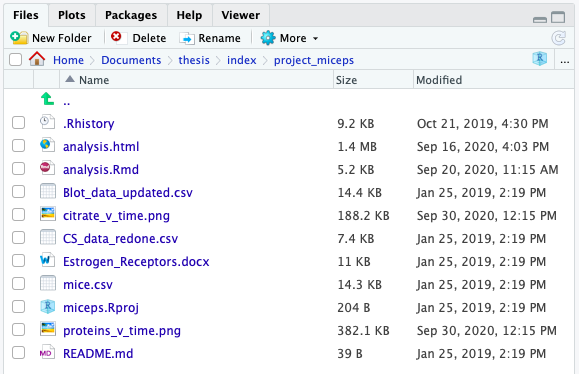
\includegraphics[width=1\linewidth]{figure/sample-project} \caption{A Sample R Project}\label{fig:unnamed-chunk-7}
\end{figure}
\subsection{Component 1: Accessibile Project
Files}\label{component-1-accessibile-project-files}
\begin{Shaded}
\begin{Highlighting}[]
\KeywordTok{library}\NormalTok{(fertile)}
\end{Highlighting}
\end{Shaded}
\texttt{fertile} takes several steps to help users ensure that all of
files necessary to run an analysis are provided in the project folder.

\subsubsection{File Overview}\label{file-overview}

One of the fastest ways to gain an overview of the existing files
(including data, code, and metadata) is with the
\texttt{proj\_analyze\_files()} function. It lists all of the files in
the project, along with their size, type, and relative path within the
directory. This can help users quickly produce an overview of how many
code, data, and auxilliary (image or text) files they have.
\begin{Shaded}
\begin{Highlighting}[]
\KeywordTok{proj_analyze_files}\NormalTok{(}\StringTok{"project_miceps"}\NormalTok{)}
\end{Highlighting}
\end{Shaded}
\begin{verbatim}
# A tibble: 11 x 5
   file                     size ext   mime                       path_rel      
   <fs::path>           <fs::by> <chr> <chr>                      <fs::path>    
 1 project_miceps/Blot~   14.43K csv   text/csv                   Blot_data_upd~
 2 project_miceps/CS_d~    7.39K csv   text/csv                   CS_data_redon~
 3 project_miceps/Estr~   10.97K docx  application/vnd.openxmlfo~ Estrogen_Rece~
 4 project_miceps/READ~       39 md    text/markdown              README.md     
 5 project_miceps/anal~    5.21K Rmd   text/x-markdown            analysis.Rmd  
 6 project_miceps/anal~    1.41M html  text/html                  analysis.html 
 7 project_miceps/citr~  187.75K png   image/png                  citrate_v_tim~
 8 project_miceps/mice~   14.33K csv   text/csv                   mice.csv      
 9 project_miceps/mice~      204 Rproj text/rstudio               miceps.Rproj  
10 project_miceps/prot~  378.04K png   image/png                  proteins_v_ti~
11 project_miceps/soft~    5.34K txt   text/plain                 software-vers~
\end{verbatim}
Users can also check for the existence of a README description file with
\texttt{has\_readme()}:
\begin{Shaded}
\begin{Highlighting}[]
\KeywordTok{has_readme}\NormalTok{(}\StringTok{"project_miceps"}\NormalTok{)}
\end{Highlighting}
\end{Shaded}
\begin{verbatim}
v Checking for README file(s) at root level
\end{verbatim}
\subsubsection{Testing For
Self-Containment}\label{testing-for-self-containment}

In order to truly check that a project is self contained, however, is is
necessary to remove it from the environment it is located, ensuring that
it can still run when cut off from the main file system.

The \texttt{sandbox()} function is designed to help facilitate this.
\texttt{sandbox()} allows the user to make a copy of their project in a
temporary directory that is isolated from the file system.
\begin{Shaded}
\begin{Highlighting}[]
\NormalTok{fs}\OperatorTok{::}\KeywordTok{dir_ls}\NormalTok{(}\StringTok{'project_miceps'}\NormalTok{) }\OperatorTok\StringTok{ }\KeywordTok{head}\NormalTok{(}\DecValTok{3}\NormalTok{)}
\end{Highlighting}
\end{Shaded}
\begin{verbatim}
project_miceps/Blot_data_updated.csv   project_miceps/CS_data_redone.csv      
project_miceps/Estrogen_Receptors.docx 
\end{verbatim}
\begin{Shaded}
\begin{Highlighting}[]
\NormalTok{temp_dir <-}\StringTok{ }\KeywordTok{sandbox}\NormalTok{(}\StringTok{'project_miceps'}\NormalTok{)}
\NormalTok{temp_dir}
\end{Highlighting}
\end{Shaded}
\begin{verbatim}
/var/folders/v6/f62qz88s0sd5n3yqw9d8sb300000gn/T/RtmpuaH9Oz/project_miceps
\end{verbatim}
\begin{Shaded}
\begin{Highlighting}[]
\NormalTok{fs}\OperatorTok{::}\KeywordTok{dir_ls}\NormalTok{(temp_dir) }\OperatorTok\StringTok{ }\KeywordTok{head}\NormalTok{(}\DecValTok{3}\NormalTok{)}
\end{Highlighting}
\end{Shaded}
\begin{verbatim}
/var/folders/v6/f62qz88s0sd5n3yqw9d8sb300000gn/T/RtmpuaH9Oz/project_miceps/Blot_data_updated.csv
/var/folders/v6/f62qz88s0sd5n3yqw9d8sb300000gn/T/RtmpuaH9Oz/project_miceps/CS_data_redone.csv
/var/folders/v6/f62qz88s0sd5n3yqw9d8sb300000gn/T/RtmpuaH9Oz/project_miceps/Estrogen_Receptors.docx
\end{verbatim}
Once a directory is sandboxed, users can run the \texttt{proj\_render()}
function, which checks all \texttt{.R} and \texttt{.Rmd} code files in
the directory to ensure that they can compile properly, to ensure that
their project is self-contained.
\begin{Shaded}
\begin{Highlighting}[]
\KeywordTok{proj_render}\NormalTok{(temp_dir)}
\end{Highlighting}
\end{Shaded}
\begin{verbatim}
-- Rendering R scripts... ------------------------------------------------------- fertile 0.0.0.9027 --
\end{verbatim}
\begin{verbatim}
Warning: `data_frame()` is deprecated as of tibble 1.1.0.
Please use `tibble()` instead.
This warning is displayed once every 8 hours.
Call `lifecycle::last_warnings()` to see where this warning was generated.
\end{verbatim}
If \texttt{proj\_render()} executes without error, this indicates that
all the necessary files are present. Users can also confirm this by
checking the time stamp of the last successful render, captured in the
\texttt{render\_log\_report()} function. If the time stamp matches the
current time, the project successfully compiled.
\begin{Shaded}
\begin{Highlighting}[]
\KeywordTok{slice_tail}\NormalTok{(}\KeywordTok{render_log_report}\NormalTok{(temp_dir))}
\end{Highlighting}
\end{Shaded}
\begin{verbatim}
Reading from /var/folders/v6/f62qz88s0sd5n3yqw9d8sb300000gn/T/RtmpuaH9Oz/project_miceps/.fertile_render_log.csv
\end{verbatim}
\begin{verbatim}
# A tibble: 1 x 4
  path          path_abs func        timestamp          
  <chr>         <chr>    <chr>       <dttm>             
1 LAST RENDERED <NA>     proj_render 2020-10-05 14:16:32
\end{verbatim}
What we \emph{need}:
\begin{itemize}
\tightlist
\item
  can we report a checklist of the types of files we have available?
\item
  it should check for the existence of a code file and data file and
  also readme
\end{itemize}
\subsection{Component 2: Organized Project
Structure}\label{component-2-organized-project-structure}

\texttt{fertile} provides a wide variety of features for managing the
file system of a project. Nine of the package's fifteen primary
reproducibility checks relate to file structure.

\subsubsection{Clear Project Root}\label{clear-project-root}

Two of these are focused on the \texttt{R\ project} aspect of the file
system. \texttt{has\_proj\_root()} ensures that there is a single
\texttt{.Rproj} file indicating a clear root directory for the project,
while \texttt{has\_no\_nested\_proj\_root()} ensures that there are no
sub-projects within. The recognition of a clear root directory is
necessary to allow for file structure analysis and project restructuring
as it provides a baseline directory to define relative file paths from.

\subsubsection{No File Clutter}\label{no-file-clutter}

Six of the major checks, whose names begin with \texttt{has\_tidy\_}
focus on file clutter, addressing one of the components of a clean file
structure. They check to make sure that no audio/video, image, source,
raw data, .rda, or .R files are found in the root directory of the
project.

The last check that focuses on the file system is
\texttt{has\_only\_used\_files()}. One of the more complicated checks in
\texttt{fertile}, this function checks to make sure that there are no
extraneous files serving no purpose (that are not ``used'') included
alongside the analysis. For this function to work properly, a clear
definition of which files are considered as ``used'' is needed. In
\texttt{fertile}, that definition includes the following:
\begin{itemize}
\tightlist
\item
  \texttt{.R},\texttt{.Rmd}, and \texttt{.Rproj} files
\item
  README files
\item
  Data/text/image files whose file path is referenced, either as an
  input or output, in any of the \texttt{.R} or \texttt{.Rmd} files
\item
  Outputs created by knitting any \texttt{.Rmd} files (\texttt{.html},
  \texttt{.pdf}, or \texttt{.docx} files with the same name as the
  \texttt{.Rmd})
\item
  Files created by \texttt{fertile}. In an effort to capture information
  about dependencies, \texttt{fertile} creates a text file capturing the
  session information when a project is run and provides an option to
  generate an \texttt{.R} script that can install all of the packages
  referenced in a project's code. These files are considered ``used.''
\end{itemize}
\begin{Shaded}
\begin{Highlighting}[]
\CommentTok{# List the files in the directory}
\NormalTok{fs}\OperatorTok{::}\KeywordTok{dir_ls}\NormalTok{(}\StringTok{"project_miceps"}\NormalTok{)}
\end{Highlighting}
\end{Shaded}
\begin{verbatim}
project_miceps/Blot_data_updated.csv   project_miceps/CS_data_redone.csv      
project_miceps/Estrogen_Receptors.docx project_miceps/README.md               
project_miceps/analysis.Rmd            project_miceps/analysis.html           
project_miceps/citrate_v_time.png      project_miceps/mice.csv                
project_miceps/miceps.Rproj            project_miceps/proteins_v_time.png     
project_miceps/software-versions.txt   
\end{verbatim}
\begin{Shaded}
\begin{Highlighting}[]
\CommentTok{# Check to see which are "used"}
\KeywordTok{has_only_used_files}\NormalTok{(}\StringTok{"project_miceps"}\NormalTok{)}
\end{Highlighting}
\end{Shaded}
\begin{verbatim}
Joining, by = "path_abs"
\end{verbatim}
\begin{verbatim}
* Checking to see if all files in directory are used in code
\end{verbatim}
\begin{verbatim}
   Problem: You have files in your project directory which are not being used.
\end{verbatim}
\begin{verbatim}
   Solution: Use or delete files.
\end{verbatim}
\begin{verbatim}
   See for help: ?fs::file_delete
\end{verbatim}
\begin{verbatim}
# A tibble: 2 x 1
  path_abs                                                                      
  <chr>                                                                         
1 /Users/audreybertin/Documents/thesis/index/project_miceps/Estrogen_Receptors.~
2 /Users/audreybertin/Documents/thesis/index/project_miceps/mice.csv            
\end{verbatim}
\subsubsection{Reorganizing File
Structure}\label{reorganizing-file-structure}

There are also several functions help with reshaping the entire project
structure to a more reproducibile format. For example,
\texttt{proj\_suggest\_moves()} provides suggestions for how to
reorganize the files into folders.
\begin{Shaded}
\begin{Highlighting}[]
\NormalTok{files <-}\StringTok{ }\KeywordTok{proj_analyze_files}\NormalTok{(}\StringTok{"project_miceps"}\NormalTok{)}

\KeywordTok{proj_suggest_moves}\NormalTok{(files)}
\end{Highlighting}
\end{Shaded}
\begin{verbatim}
# A tibble: 9 x 8
  file             size ext   mime     path_rel   dir_rel    path_new    cmd    
  <fs::path>   <fs::by> <chr> <chr>    <fs::path> <fs::path> <fs::path>  <chr>  
1 project_mic~   14.43K csv   text/csv Blot_data~ data-raw   project_mi~ file_m~
2 project_mic~    7.39K csv   text/csv CS_data_r~ data-raw   project_mi~ file_m~
3 project_mic~   10.97K docx  applica~ Estrogen_~ inst/other project_mi~ file_m~
4 project_mic~    5.21K Rmd   text/x-~ analysis.~ vignettes  project_mi~ file_m~
5 project_mic~    1.41M html  text/ht~ analysis.~ inst/text  project_mi~ file_m~
6 project_mic~  187.75K png   image/p~ citrate_v~ inst/image project_mi~ file_m~
7 project_mic~   14.33K csv   text/csv mice.csv   data-raw   project_mi~ file_m~
8 project_mic~  378.04K png   image/p~ proteins_~ inst/image project_mi~ file_m~
9 project_mic~    5.34K txt   text/pl~ software-~ inst/text  project_mi~ file_m~
\end{verbatim}
These suggestions are based on achieving the optimal file structure
design for reproducibility, argued by Marwick et al. (2018) to be that
of an \texttt{R} package (R-Core-Team (2020), Wickham (2015)), with an
\texttt{R} folder, as well as \texttt{data}, \texttt{data-raw},
\texttt{inst}, and \texttt{vignettes}. Such a structure keeps all of the
files separated and in clearly labeled directories where they are easy
to find. Additionally, the extension of the \texttt{R} package structure
to data analysis projects promotes standardization of file structure
within the R community.

Users can execute these suggestions individually, using the code
snippets provided next to each file name when running
\texttt{proj\_suggest\_moves()}, but they can also run them all
together. \texttt{proj\_move\_files()} executes all of the suggestions
from \texttt{proj\_suggest\_moves()} at once, building an \texttt{R}
package style structure and sorting files into the correct folders by
type.

Combined together, all of these functions make it simple to ensure that
projects fall under a standard, simple, and reproducible structure with
minimal clutter.

\subsection{Component 3: Documentation}\label{component-3-documentation}

High quality documentation, including the presence of a README file,
comments explaining the code, a list of software packages an analysis is
dependent on, and a method in which to understand which order to run
code files in, is incredibly important to reproducibility. Without
written guidance, individuals looking to reproduce results may not
understand how to take all of the project components and combine them in
the right way to produce the desired outcome. Additionally, code used
without the proper dependencies and software versions, even if it is
perfectly functional and correctly written, will often result in errors
when compiled.

\texttt{fertile} contains a variety of functions to ensure that projects
are well documented.

\subsubsection{README}\label{readme}

One important component of documentation is the inclusion of a README
file. A README is a text file that introduces and explains a project.
Commonly, a project README contains background information necessary to
understand a project. Some of the components that might be contained
within are:
\begin{enumerate}
\def\labelenumi{\arabic{enumi}.}
\tightlist
\item
  Background on the purpose of the project and the questions of
  interest.
\item
  Background on where the data used in the project came from and what
  they contain.
\item
  Information about installing and setting up the software necessary to
  run it.
\item
  A list of included files.
\item
  A description of how to run the project---for example, a summary of
  the order in which the included files should be run.
\item
  Contact information for the author of the project.
\end{enumerate}
\texttt{fertile} ensures that a README is included alongside the user's
project with the \texttt{has\_readme()} function:
\begin{Shaded}
\begin{Highlighting}[]
\KeywordTok{has_readme}\NormalTok{(}\StringTok{"project_miceps"}\NormalTok{)}
\end{Highlighting}
\end{Shaded}
\begin{verbatim}
v Checking for README file(s) at root level
\end{verbatim}
\subsubsection{Clear File Order}\label{clear-file-order}

Another important component of documentation is that it must be clear in
which order provided files should be run. While this information can be
included as part of the README, it is sometimes provided via other
methods---for example, through a \texttt{makefile}/\texttt{drakefile}
(make-style file generated by the \texttt{Drake} package in \texttt{R})
or through a standardized naming or numbering convention of files.

\texttt{has\_clear\_build\_chain()} checks for these non-README methods
of ensuring that file ordering is clear. \texttt{project\_miceps}, since
it only contains one code file, passes this check easily:
\begin{Shaded}
\begin{Highlighting}[]
\KeywordTok{has_clear_build_chain}\NormalTok{(}\StringTok{"project_miceps"}\NormalTok{)}
\end{Highlighting}
\end{Shaded}
\begin{verbatim}
v Checking for clear build chain
\end{verbatim}
\subsubsection{Software Dependencies}\label{software-dependencies}

There are also several features focused on software dependencies. Every
time the code contained within a project is rendered by
\texttt{fertile}, the package generates a file capturing the
\texttt{sessionInfo()} just after the code was run. This file contains
information about the R version in which the code was run, the list of
packages that were loaded, and their specific versions.

The dependency information from \texttt{project\_miceps} looks as
follows:
\begin{verbatim}
-- Rendering R scripts... ------------------------------------------------------- fertile 0.0.0.9027 --
\end{verbatim}
\begin{Shaded}
\begin{Highlighting}[]
\NormalTok{session_info <-}\StringTok{ "project_miceps/.software-versions.txt"}
\KeywordTok{cat}\NormalTok{(}\KeywordTok{readChar}\NormalTok{(session_info, }\FloatTok{1e5}\NormalTok{))}
\end{Highlighting}
\end{Shaded}
\begin{verbatim}
The R project located at '/Users/audreybertin/Documents/thesis/index/project_miceps' was last run in the following software environment:


R version 4.0.2 (2020-06-22)
Platform: x86_64-apple-darwin17.0 (64-bit)
Running under: macOS Catalina 10.15.5

Matrix products: default
BLAS:   /Library/Frameworks/R.framework/Versions/4.0/Resources/lib/libRblas.dylib
LAPACK: /Library/Frameworks/R.framework/Versions/4.0/Resources/lib/libRlapack.dylib

locale:
en_US.UTF-8/en_US.UTF-8/en_US.UTF-8/C/en_US.UTF-8/en_US.UTF-8

attached base packages:
stats     graphics  grDevices utils     datasets  methods   base     

other attached packages:
stargazer_5.2.2    skimr_2.1.2        purrr_0.3.4       
ggplot2_3.3.2      tidyr_1.1.2        readr_1.3.1        dplyr_1.0.2       
\end{verbatim}
Interactively, users can access this dependency summary using the
function \texttt{proj\_dependency\_report()}.

The \texttt{proj\_pkg\_script()} function builds off of this behavior,
providing a method to simplify the process of installing the packages
seen in the dependency report.

When run on an \texttt{R} project directory, the function creates a
\texttt{.R} script file that contains the code needed to install all of
the packages referenced in the project, differentiating between packages
located on CRAN and those located on GitHub.
\begin{Shaded}
\begin{Highlighting}[]
\NormalTok{install_script <-}\StringTok{ }\KeywordTok{proj_pkg_script}\NormalTok{(}\StringTok{"project_miceps"}\NormalTok{)}
\KeywordTok{cat}\NormalTok{(}\KeywordTok{readChar}\NormalTok{(install_script, }\FloatTok{1e5}\NormalTok{))}
\end{Highlighting}
\end{Shaded}
\begin{verbatim}
# Run this script to install the required packages for this
R project.
# Packages hosted on CRAN...
install.packages(c( 'broom', 'dplyr', 'fs', 'ggplot2',
'purrr', 'readr', 'rmarkdown', 'skimr', 'stargazer',
'tidyr' ))
# Packages hosted on GitHub...
\end{verbatim}
Users interested in ensuring that their project is reproducible can
provide alongside it both:
\begin{enumerate}
\def\labelenumi{\arabic{enumi}.}
\tightlist
\item
  The text-based summary of dependencies produced by
  \texttt{proj\_dependency\_report()}.
\item
  The \texttt{.R} dependency installation script.
\end{enumerate}
Then, anyone wanting to re-create the results would have the
documentation necessary to do so alongside a quick and easy method to
set up the required software.

\subsubsection{Code Commenting}\label{code-commenting}

In addition to README and dependency documentation, \texttt{fertile}
also analyzes the quality of documentation provided directly alongside
code.

Code commenting---the process of placing human-readable descriptions
next to code to explain what the code is doing---is incredibly important
for ensuring that a project can be understood by someone other than its
author. To ensure that their code is understandable, data analysts must
regularly include comments throughout their project code files.

\texttt{has\_well\_commented\_code()} is designed to check for this. The
function reads through all \texttt{.R} and \texttt{.Rmd} files in a
project directory and, for each, calculates the fraction of lines in the
file that are comments. Files for which comments make up less than 10\%
of the written lines are flagged as poorly commented, warning users to
make corrections and increase the number of comments in their code.

The primary code file in \texttt{project\_miceps}, ``analysis.Rmd'', is
a great example of a poorly commented file. It only contains 6 lines of
comments, while including over 100 lines of code. As such, it is flagged
by \texttt{has\_well\_commented\_code()}:
\begin{Shaded}
\begin{Highlighting}[]
\KeywordTok{has_well_commented_code}\NormalTok{(}\StringTok{"project_miceps"}\NormalTok{)}
\end{Highlighting}
\end{Shaded}
\begin{verbatim}
* Checking that code is adequately commented
\end{verbatim}
\begin{verbatim}
   Problem: Poorly commented .R or .Rmd files found
\end{verbatim}
\begin{verbatim}
   Solution: Add more comments to the files below. At least 10% of the lines should be comments.
\end{verbatim}
\begin{verbatim}
   See for help: https://intelligea.wordpress.com/2013/06/30/inline-and-block-comments-in-r/
\end{verbatim}
\begin{verbatim}
# A tibble: 1 x 2
  file_name                   fraction_lines_commented
  <chr>                                          <dbl>
1 project_miceps/analysis.Rmd                     0.04
\end{verbatim}
What we \emph{need}:
\begin{itemize}
\tightlist
\item
  possibly a makefile generator? or improvements to order checking?
\end{itemize}
\subsection{Component 4: File Paths}\label{component-4-file-paths}

\texttt{fertile} contains a variety of features designed to address
issues with file paths. Several of these features happen proactively,
warning users that they are entering a non-reproducible file path as it
happens, while others can be accessed after a project has already been
written.

\subsubsection{Proactive Warnings When
Coding}\label{proactive-warnings-when-coding}

Proactively, \texttt{fertile} catches when an absolute path, or one
leading outside of the project directory, is referenced in an input or
output function and outputs a warning message. This interactive behavior
is one of the educational features of the package, as it immediately
provides an informative message explaining what went wrong, giving the
programmer an opportunity to learn and course-correct from there.
\begin{Shaded}
\begin{Highlighting}[]
\KeywordTok{library}\NormalTok{(fertile)}
\KeywordTok{file.exists}\NormalTok{(}\StringTok{"~/Desktop/my_data.csv"}\NormalTok{)}
\end{Highlighting}
\end{Shaded}
\begin{verbatim}
[1] TRUE
\end{verbatim}
\begin{Shaded}
\begin{Highlighting}[]
\KeywordTok{read.csv}\NormalTok{(}\StringTok{"~/Desktop/my_data.csv"}\NormalTok{)}
\end{Highlighting}
\end{Shaded}
\begin{verbatim}
Error: Detected absolute paths
\end{verbatim}
\begin{Shaded}
\begin{Highlighting}[]
\KeywordTok{read.csv}\NormalTok{(}\StringTok{"../../../Desktop/my_data.csv"}\NormalTok{)}
\end{Highlighting}
\end{Shaded}
\begin{verbatim}
Error: Detected paths that lead outside the project directory
\end{verbatim}
\texttt{fertile} is particularly strict with the function
\texttt{setwd()}, as its use is almost certain to break reproducibility.
Calls to \texttt{setwd()} are blocked from executing, and users must
conduct a manual override, via the \texttt{danger()} function, to change
their working directory.
\begin{Shaded}
\begin{Highlighting}[]
\KeywordTok{getwd}\NormalTok{()}
\end{Highlighting}
\end{Shaded}
\begin{verbatim}
[1] "/Users/audreybertin/Documents/thesis/index"
\end{verbatim}
\begin{Shaded}
\begin{Highlighting}[]
\KeywordTok{setwd}\NormalTok{(}\StringTok{"~/Desktop"}\NormalTok{)}
\end{Highlighting}
\end{Shaded}
\begin{verbatim}
Error: setwd() is likely to break reproducibility. Use here::here() instead.
\end{verbatim}
\begin{Shaded}
\begin{Highlighting}[]
\KeywordTok{getwd}\NormalTok{()}
\end{Highlighting}
\end{Shaded}
\begin{verbatim}
[1] "/Users/audreybertin/Documents/thesis/index"
\end{verbatim}
\subsubsection{Project Path Summaries}\label{project-path-summaries}

\texttt{fertile} also contains functionality that analyzes code for path
information after it is written. For example,
\texttt{proj\_analyze\_paths} goes through all of the paths used in a
project's \texttt{.R} and \texttt{.Rmd} files and produces a report
detailing which ones failed to meet reproducibility standards,
explaining the problem, and providing a solution.
\begin{Shaded}
\begin{Highlighting}[]
\KeywordTok{proj_analyze_paths}\NormalTok{(}\StringTok{'project_miceps'}\NormalTok{)}
\end{Highlighting}
\end{Shaded}
\begin{verbatim}
-- Generating reproducibility report... ----------------------------------------- fertile 0.0.0.9027 --
\end{verbatim}
\begin{verbatim}
Checking for absolute paths...
\end{verbatim}
\begin{verbatim}
Checking for paths outside project directory...
\end{verbatim}
\begin{verbatim}
New names:
* path -> path...1
* path -> path...5
\end{verbatim}
\begin{verbatim}
# A tibble: 2 x 6
  path...1        path_abs        func   path...5       problem     solution    
  <chr>           <chr>           <chr>  <chr>          <chr>       <chr>       
1 /Users/audreyb~ /Users/audreyb~ readr~ /Users/audrey~ Absolute p~ Use a relat~
2 /Users/audreyb~ /Users/audreyb~ readr~ /Users/audrey~ Path is no~ Move the fi~
\end{verbatim}
Paths can also be checked individually, or in groups, using
\texttt{check\_path()}.
\begin{Shaded}
\begin{Highlighting}[]
\CommentTok{# Path inside the directory}
\KeywordTok{check_path}\NormalTok{(}\StringTok{"project_miceps"}\NormalTok{)}
\end{Highlighting}
\end{Shaded}
\begin{verbatim}
# A tibble: 0 x 3
# ... with 3 variables: path <chr>, problem <chr>, solution <chr>
\end{verbatim}
\begin{Shaded}
\begin{Highlighting}[]
\CommentTok{# Absolute path (current working directory)}
\KeywordTok{check_path}\NormalTok{(}\KeywordTok{getwd}\NormalTok{())}
\end{Highlighting}
\end{Shaded}
\begin{verbatim}
Error: Detected absolute paths
\end{verbatim}
\begin{Shaded}
\begin{Highlighting}[]
\CommentTok{# Path outside the directory}
\KeywordTok{check_path}\NormalTok{(}\StringTok{"../README.md"}\NormalTok{)}
\end{Highlighting}
\end{Shaded}
\begin{verbatim}
Error: Detected paths that lead outside the project directory
\end{verbatim}
These functions, together, cover all of the reproducibility
subcomponents involving file paths. Users are warned not to use absolute
paths or paths pointing outside of the directory, both while they are
coding and after the fact, and provided with a recommended solution to
the problem if they do so. Additionally, users are prevented from using
functions that will certainly break reproducibility and provided with
safer alternatives.

\subsection{Component 5: Randomness}\label{component-5-randomness}

The component of randomness is addressed by \texttt{fertile} in a
reproducibility check function titled \texttt{has\_no\_randomness()},
which does the following: First, it checks code files to determine
whether they have employed random number generation. This is confirmed
by recording the random number generation seed prior to running the
files, rendering the files, and then checking to see whether the seed
has changed. If the seed has changed, that indicates that random number
generation has occurred. Then, it determines whether whether any
randomness present was semi-random (i.e.~controlled and repeatable) or
truly random, by checking whether the \texttt{set.seed()} function was
called. If the randomness was semi-random, it is considered permissible
and reproducible. Truly random code is flagged as dangerous.

Let us consider an example from \texttt{project\_miceps}. The primary
code file, \texttt{analysis.Rmd} contains the following code. In this
code, we see that a data set is read in via \texttt{read\_csv} and
reformatted. Then, the \texttt{sample\_frac()} function takes a random
sample of 50\% of the rows of the data.
\begin{Shaded}
\begin{Highlighting}[]
\NormalTok{mice <-}\StringTok{ }\KeywordTok{read_csv}\NormalTok{(}\StringTok{"Blot_data_updated.csv"}\NormalTok{) }\OperatorTok
\StringTok{  }\KeywordTok{transmute}\NormalTok{(}\DataTypeTok{time =} \StringTok{`}\DataTypeTok{Time point}\StringTok{`}\NormalTok{,}
            \DataTypeTok{sex =}\NormalTok{ Sex,}
            \DataTypeTok{id =} \StringTok{`}\DataTypeTok{Mouse #}\StringTok{`}\NormalTok{,}
            \DataTypeTok{erb =} \StringTok{`}\DataTypeTok{ERB Normalized Final}\StringTok{`}\NormalTok{,}
            \DataTypeTok{era =} \StringTok{`}\DataTypeTok{ERA Normalized Final}\StringTok{`}\NormalTok{,}
            \DataTypeTok{gper =} \StringTok{`}\DataTypeTok{GPER Normalized Final}\StringTok{`}\NormalTok{) }\OperatorTok
\StringTok{  }\KeywordTok{mutate}\NormalTok{(}\DataTypeTok{day =} \KeywordTok{case_when}\NormalTok{(}
\NormalTok{    time }\OperatorTok{==}\StringTok{ }\DecValTok{0} \OperatorTok{~}\StringTok{ }\OperatorTok{-}\DecValTok{1}\NormalTok{,}
\NormalTok{    time }\OperatorTok{==}\StringTok{ }\DecValTok{1} \OperatorTok{~}\StringTok{ }\DecValTok{0}\NormalTok{,}
\NormalTok{    time }\OperatorTok{==}\StringTok{ }\DecValTok{2} \OperatorTok{~}\StringTok{ }\DecValTok{1}\NormalTok{,}
\NormalTok{    time }\OperatorTok{==}\StringTok{ }\DecValTok{3} \OperatorTok{~}\StringTok{ }\DecValTok{3}\NormalTok{,}
\NormalTok{    time }\OperatorTok{==}\StringTok{ }\DecValTok{4} \OperatorTok{~}\StringTok{ }\DecValTok{5}\NormalTok{,}
\NormalTok{    time }\OperatorTok{==}\StringTok{ }\DecValTok{5} \OperatorTok{~}\StringTok{ }\DecValTok{7}
\NormalTok{  ),}
  \DataTypeTok{type =} \KeywordTok{ifelse}\NormalTok{(time }\OperatorTok{==}\StringTok{ }\DecValTok{0}\NormalTok{, }\StringTok{"control"}\NormalTok{, }\StringTok{"treatment"}\NormalTok{)}
\NormalTok{  )}
\NormalTok{mice_tidy <-}\StringTok{ }\NormalTok{mice }\OperatorTok
\StringTok{  }\KeywordTok{select}\NormalTok{(}\OperatorTok{-}\NormalTok{time) }\OperatorTok
\StringTok{  }\KeywordTok{gather}\NormalTok{(}\DataTypeTok{key =} \StringTok{"protein"}\NormalTok{, }\DataTypeTok{value =} \StringTok{"amount"}\NormalTok{, }\OperatorTok{-}\NormalTok{day, }\OperatorTok{-}\NormalTok{sex, }\OperatorTok{-}\NormalTok{id, }\OperatorTok{-}\NormalTok{type) }\OperatorTok
\StringTok{  }\KeywordTok{mutate}\NormalTok{(}\DataTypeTok{protein_label =} \KeywordTok{factor}\NormalTok{(protein,}
    \DataTypeTok{labels =} \KeywordTok{c}\NormalTok{(}\StringTok{"paste(ER, alpha)"}\NormalTok{, }\StringTok{"paste(ER, beta)"}\NormalTok{, }\StringTok{"GPER"}\NormalTok{)))}
\end{Highlighting}
\end{Shaded}
\begin{Shaded}
\begin{Highlighting}[]
\KeywordTok{sample_frac}\NormalTok{(mice, }\FloatTok{0.5}\NormalTok{)}
\end{Highlighting}
\end{Shaded}
However, there is no seed set in the file. As a result,
\texttt{has\_no\_randomness()} returns as a failure for the project. Had
a seed been set, however, the project would have passed.
\begin{Shaded}
\begin{Highlighting}[]
\KeywordTok{has_no_randomness}\NormalTok{(}\StringTok{'project_miceps'}\NormalTok{)}
\end{Highlighting}
\end{Shaded}
\begin{verbatim}
* Checking for no randomness
\end{verbatim}
\begin{verbatim}
   Problem: Your code uses randomness
\end{verbatim}
\begin{verbatim}
   Solution: Set a seed using `set.seed()` to ensure reproducibility.
\end{verbatim}
\begin{verbatim}
   See for help: ?set.seed
\end{verbatim}
\begin{verbatim}
# A tibble: 1 x 2
  culprit expr                
  <chr>   <glue>              
1 ?       Example: set.seed(1)
\end{verbatim}
\texttt{fertile}'s randomness-centered feature helps analysts know that
their use of randomness is controlled, ensuring that functions involving
random number generation will always produce the same output each time
they are run.

\subsection{Component 6: Readability and
Style}\label{component-6-readability-and-style}

Though not an absolutely necessary component of reproducibility, code
style can have a significant impact on how easy it is to follow the
steps being taken in an analysis. The use of consistent and
highly-readable style in code greatly simplifies and speeds up the
process of understanding a data analysis project and repeating the steps
included within.

\texttt{fertile} addresses code style via the function
\texttt{has\_no\_lint()}. This function checks code for compatibility
with RStudio Chief Scientist Hadley Wikham's ``tidy'' code format, which
promotes the following best practices:
\begin{itemize}
\tightlist
\item
  Line length should not exceed 80 characters
\item
  There should not be trailing whitespace
\item
  All infix operators (\texttt{=}, \texttt{+}, \texttt{-},
  \texttt{\textless{}-}, etc) should have spaces on either side
\item
  All commas should be followed by spaces
\item
  There is no code left in the file that is commented out
\item
  \texttt{\textless{}-} should be used instead of \texttt{=} to assign
  variables
\item
  Opening curly braces should never go on their own line and should
  always be followed by a new line
\item
  There should always be a space between right parenthesis and an open
  curly brace
\item
  Closing curly braces should always be on their own line, unless
  followed by an \texttt{else} statement
\end{itemize}
Any issues with incompatibility that are found by
\texttt{has\_no\_lint()} appear in a window by the RStudio console. This
window lists the style inconsistencies found in each code document,
showing both the description of the error and the line number where it
occurred for each issue. This window is interactive; double-clicking on
an error brings the user to exact location in the code where it
occurred.

Let us consider an example. \texttt{project\_miceps} contains an
\texttt{RMarkdown} file titled \texttt{analysis.Rmd}, which contains
some code involved with a data analysis. Some of the code is in tidy
style but not all of it is.

For example, line 71, part of a \texttt{ggplot} call, contains the
following code:
\begin{Shaded}
\begin{Highlighting}[]
\CommentTok{# Line 71 of `project_miceps/analysis.Rmd'}

\KeywordTok{geom_hline}\NormalTok{(}\KeywordTok{aes}\NormalTok{(}\DataTypeTok{yintercept =}\NormalTok{ estimate }\OperatorTok{+}\StringTok{ }\FloatTok{1.96}\OperatorTok{*}\NormalTok{std.error, }\DataTypeTok{color =}\NormalTok{ sex), }\DataTypeTok{linetype =} \DecValTok{3}\NormalTok{) }\OperatorTok{+}\StringTok{ }
\end{Highlighting}
\end{Shaded}
For this line, \texttt{has\_no\_lint()} finds the following
inconsistencies with tidy style:
\begin{itemize}
\item
  Line 71: Lines should not be more than 80 characters.
\item
  Line 71: Put spaces around all infix operators.
\item
  Line 71: Trailing whitespace is superfluous.
\end{itemize}
The first comes up because the true line length, including spaces, is 84
characters. The second comes up because the \texttt{*} between
\texttt{1.96} and \texttt{std.error} is not surrounded by spaces. The
third is flagged because there is an empty space after the \texttt{+} at
the end of the line.

An even less tidy piece of code is that found on line 189, written as
follows:
\begin{Shaded}
\begin{Highlighting}[]
\CommentTok{# Line 189 of `project_miceps/analysis.Rmd'}

\ControlFlowTok{if}\NormalTok{ (}\KeywordTok{length}\NormalTok{(mice) }\OperatorTok{>}\StringTok{ }\DecValTok{1}\NormalTok{)\{ holder_var =}\StringTok{ }\DecValTok{1}\NormalTok{ \}}
\end{Highlighting}
\end{Shaded}
For this line, \texttt{has\_no\_lint()} finds the following errors:
\begin{itemize}
\item
  Line 189: There should be a space between right parenthesis and an
  opening curly brace.
\item
  Line 189: Opening curly braces should never go on their own line and
  should always be followed by a new line.
\item
  Line 189: Use \textless{}-, not =, for assignment.
\item
  Line 189: Closing curly braces should always be on their own line,
  unless it's followed by an else.
\end{itemize}
The first issue flagged is the fact that \texttt{)\{}, in the middle of
the line, has no space in the middle. The second issue is flagged
because the code to execute when the \texttt{if} statement is true
(\texttt{holder\_var\ =\ 1}) is on the same line as the \texttt{if}
statement, rather than on its own line. The third error occurs because
\texttt{holder\_var} is defined using an \texttt{=}. And the fourth
occurs because the closing curly brace is on the same line as other code
rather than by itself.

These informative error messages provided by \texttt{fertile} help teach
users to use consistent, tidy style in their code. They do so while
making the learning process incredibly simple, allowing users to click
and see exactly which symbol or character caused the error. In addition
to providing a detailed explanation of the was in which the provided
code is not tidy, \texttt{fertile} also suggests a simple and fast
solution for resolving the inconsistencies all at once, recommending
that users apply the \texttt{usethis::use\_tidy\_style()} function to
format their code automatically.

\subsection{Summary of Reproducibility
Components}\label{summary-of-reproducibility-components}

As described in the previous sections, \texttt{fertile} addresses all
six major components of reproducibility via a variety of functions. Some
complex components have many associated functions attached to them,
while others only have one.

A summary of the six components of reproducibility and the
functionalities in \texttt{fertile} associated with them is provided
below.
\begin{figure}
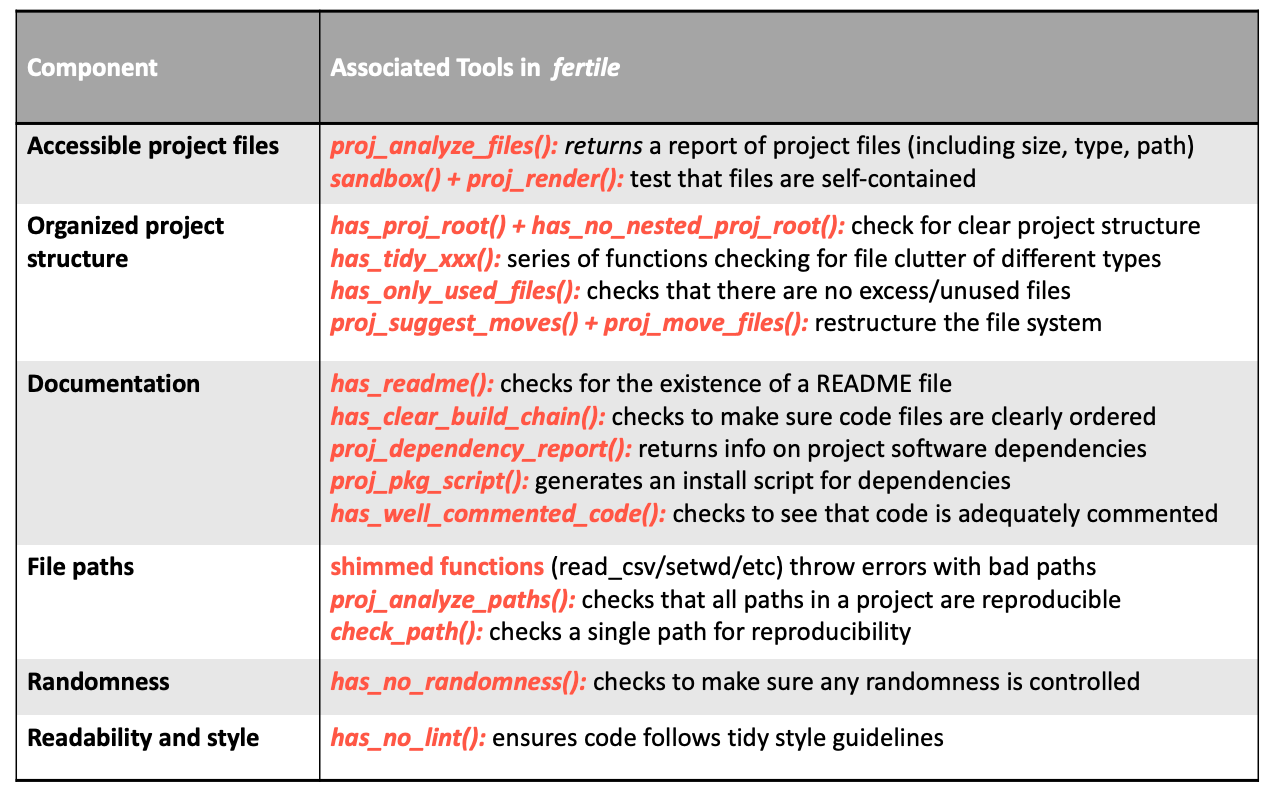
\includegraphics[width=1\linewidth]{figure/components-summary} \caption{Summary of Reproducibility Components and the Related Functionalities in 'fertile'}\label{fig:unnamed-chunk-30}
\end{figure}
\subsection{User Customizability}\label{user-customizability}

\texttt{fertile} does not force its users into a box, instead allowing
for a great deal of user choice in terms of which aspects of
reproducibility to focus on. Users can run reproducibility tests at
three different scales:
\begin{enumerate}
\def\labelenumi{\arabic{enumi})}
\item
  Comprehensively, where all checks are run within a single function or
  two.
\item
  In groups, where functions focused on similar aspects of
  reproducibility are run together.
\item
  Individually, where only one reproducbility check is run at a time.
\end{enumerate}
Users who want comprehensive behavior can access it through two primary
functions, \texttt{proj\_check()} and \texttt{proj\_analyze()}.

The \texttt{proj\_check()} function runs all fifteen reproducibility
tests in the package, noting which ones passed, which ones failed, the
reason for failure, a recommended solution, and a guide to where to look
for help. These tests, many of which were described in detail
previously, include: looking for a clear build chain, checking to make
sure the root level of the project is clear of clutter, confirming that
there are no files present that are not being directly used by or
created by the code, and looking for uses of randomness that do not have
a call to \texttt{set.seed()} present. A full list is provided below:
\begin{Shaded}
\begin{Highlighting}[]
\KeywordTok{list_checks}\NormalTok{()}
\end{Highlighting}
\end{Shaded}
\begin{verbatim}
-- The available checks in `fertile` are as follows: ---------------------------- fertile 0.0.0.9027 --
\end{verbatim}
\begin{verbatim}
 [1] "has_tidy_media"          "has_tidy_images"        
 [3] "has_tidy_code"           "has_tidy_raw_data"      
 [5] "has_tidy_data"           "has_tidy_scripts"       
 [7] "has_readme"              "has_no_lint"            
 [9] "has_proj_root"           "has_no_nested_proj_root"
[11] "has_only_used_files"     "has_clear_build_chain"  
[13] "has_no_absolute_paths"   "has_only_portable_paths"
[15] "has_no_randomness"       "has_well_commented_code"
\end{verbatim}
The \texttt{proj\_analyze()} function creates a report documenting the
structure of a data analysis project, combining four key functions from
\texttt{fertile} into one complete unit:
\begin{itemize}
\tightlist
\item
  \texttt{proj\_analyze\_packages()}, which captures a list of all
  packages referenced in the source code and which files they were
  referenced in
\item
  \texttt{proj\_analyze\_files()}, which captures a list of all of the
  files located in the directory along with their type and size
\item
  \texttt{proj\_suggest\_moves()}, which provides suggestions for how to
  reorganize files to create a more reproducible file structure
\item
  \texttt{proj\_analyze\_paths()}, which captures a list of the
  non-reproducible file paths referenced in source code
\end{itemize}
\begin{Shaded}
\begin{Highlighting}[]
\KeywordTok{proj_analyze}\NormalTok{(}\StringTok{'project_miceps'}\NormalTok{)}
\end{Highlighting}
\end{Shaded}
\begin{verbatim}
-- Analysis of reproducibility for project_miceps ------------------------------- fertile 0.0.0.9027 --
\end{verbatim}
\begin{verbatim}
--   Packages referenced in source code ----------------------------------------- fertile 0.0.0.9027 --
\end{verbatim}
\begin{verbatim}
# A tibble: 10 x 3
   package       N used_in                    
   <chr>     <int> <chr>                      
 1 broom         1 project_miceps/analysis.Rmd
 2 dplyr         1 project_miceps/analysis.Rmd
 3 fs            1 project_miceps/analysis.Rmd
 4 ggplot2       1 project_miceps/analysis.Rmd
 5 purrr         1 project_miceps/analysis.Rmd
 6 readr         1 project_miceps/analysis.Rmd
 7 rmarkdown     1 project_miceps/analysis.Rmd
 8 skimr         1 project_miceps/analysis.Rmd
 9 stargazer     1 project_miceps/analysis.Rmd
10 tidyr         1 project_miceps/analysis.Rmd
\end{verbatim}
\begin{verbatim}
--   Files present in directory ------------------------------------------------- fertile 0.0.0.9027 --
\end{verbatim}
\begin{verbatim}
# A tibble: 11 x 4
   file               ext        size mime                                      
   <fs::path>         <chr> <fs::byt> <chr>                                     
 1 Estrogen_Receptor~ docx     10.97K application/vnd.openxmlformats-officedocu~
 2 citrate_v_time.png png     187.48K image/png                                 
 3 proteins_v_time.p~ png     377.66K image/png                                 
 4 Blot_data_updated~ csv      14.43K text/csv                                  
 5 CS_data_redone.csv csv       7.39K text/csv                                  
 6 mice.csv           csv      14.33K text/csv                                  
 7 analysis.html      html      1.41M text/html                                 
 8 README.md          md           39 text/markdown                             
 9 software-versions~ txt       5.34K text/plain                                
10 miceps.Rproj       Rproj       204 text/rstudio                              
11 analysis.Rmd       Rmd       5.21K text/x-markdown                           
\end{verbatim}
\begin{verbatim}
--   Suggestions for moving files ----------------------------------------------- fertile 0.0.0.9027 --
\end{verbatim}
\begin{verbatim}
# A tibble: 9 x 3
  path_rel           dir_rel    cmd                                             
  <fs::path>         <fs::path> <chr>                                           
1 Blot_data_updated~ data-raw   file_move('project_miceps/Blot_data_updated.csv~
2 CS_data_redone.csv data-raw   file_move('project_miceps/CS_data_redone.csv', ~
3 Estrogen_Receptor~ inst/other file_move('project_miceps/Estrogen_Receptors.do~
4 analysis.Rmd       vignettes  file_move('project_miceps/analysis.Rmd', fs::di~
5 analysis.html      inst/text  file_move('project_miceps/analysis.html', fs::d~
6 citrate_v_time.png inst/image file_move('project_miceps/citrate_v_time.png', ~
7 mice.csv           data-raw   file_move('project_miceps/mice.csv', fs::dir_cr~
8 proteins_v_time.p~ inst/image file_move('project_miceps/proteins_v_time.png',~
9 software-versions~ inst/text  file_move('project_miceps/software-versions.txt~
\end{verbatim}
\begin{verbatim}
--   Problematic paths logged --------------------------------------------------- fertile 0.0.0.9027 --
\end{verbatim}
\begin{verbatim}
NULL
\end{verbatim}
Together, \texttt{proj\_check()} and \texttt{proj\_analyze()} cover a
significant portion of all six major components of reproducibility.

Users wanting to focus on groups of checks can do so using the
\texttt{proj\_check\_some()} function. \texttt{proj\_check\_some()}
leverages helper functions from \texttt{tidyselect} (Henry \& Wickham
(2020)) to allow users to call groups of similar checks together.
\texttt{tidyselect} helpers tell \texttt{fertile} to call only the
checks whose names meet certain conditions. The helper functions that
can be passed to \texttt{proj\_check\_some()} are:
\begin{itemize}
\tightlist
\item
  \texttt{starts\_with()}: Starts with a prefix.
\item
  \texttt{ends\_with()}: Ends with a suffix.
\item
  \texttt{contains()}: Contains a literal string.
\item
  \texttt{matches()}: Matches a regular expression.
\end{itemize}
For example, a variety of checks in \texttt{fertile} focus on making
sure the project has a ``tidy'' structure--essentially that there are
not files cluttered together all in one folder. Users interested in
checking their tidyness can do so all at once using
\texttt{proj\_check\_some()} as follows:
\begin{Shaded}
\begin{Highlighting}[]
\KeywordTok{proj_check_some}\NormalTok{(}\StringTok{"project_miceps"}\NormalTok{, }\KeywordTok{contains}\NormalTok{(}\StringTok{"tidy"}\NormalTok{))}
\end{Highlighting}
\end{Shaded}
\begin{verbatim}
-- Running reproducibility checks ----------------------------------------------- fertile 0.0.0.9027 --
\end{verbatim}
\begin{verbatim}
v Checking for no *.R scripts at root level
\end{verbatim}
\begin{verbatim}
v Checking for no *.rda files at root level
\end{verbatim}
\begin{verbatim}
v Checking for no A/V files at root level
\end{verbatim}
\begin{verbatim}
* Checking for no image files at root level
\end{verbatim}
\begin{verbatim}
   Problem: Image files in root directory clutter project
\end{verbatim}
\begin{verbatim}
   Solution: Move source files to img/ directory
\end{verbatim}
\begin{verbatim}
   See for help: ?fs::file_move
\end{verbatim}
\begin{verbatim}
# A tibble: 2 x 2
  culprit                     expr                                              
  <fs::path>                  <glue>                                            
1 project_miceps/citrate_v_t~ fs::file_move('project_miceps/citrate_v_time.png'~
2 project_miceps/proteins_v_~ fs::file_move('project_miceps/proteins_v_time.png~
\end{verbatim}
\begin{verbatim}
* Checking for no raw data files at root level
\end{verbatim}
\begin{verbatim}
   Problem: Raw data files in root directory clutter project
\end{verbatim}
\begin{verbatim}
   Solution: Move raw data files to data-raw/ directory
\end{verbatim}
\begin{verbatim}
   See for help: ?fs::file_move
\end{verbatim}
\begin{verbatim}
# A tibble: 3 x 2
  culprit                     expr                                              
  <fs::path>                  <glue>                                            
1 project_miceps/Blot_data_u~ fs::file_move('project_miceps/Blot_data_updated.c~
2 project_miceps/CS_data_red~ fs::file_move('project_miceps/CS_data_redone.csv'~
3 project_miceps/mice.csv     fs::file_move('project_miceps/mice.csv', here::he~
\end{verbatim}
\begin{verbatim}
v Checking for no source files at root level
\end{verbatim}
\begin{verbatim}
-- Summary of fertile checks ---------------------------------------------------- fertile 0.0.0.9027 --
\end{verbatim}
\begin{verbatim}
v Reproducibility checks passed: 4
\end{verbatim}
\begin{verbatim}
* Reproducibility checks to work on: 2
\end{verbatim}
\begin{verbatim}
* Checking for no image files at root level
\end{verbatim}
\begin{verbatim}
   Problem: Image files in root directory clutter project
\end{verbatim}
\begin{verbatim}
   Solution: Move source files to img/ directory
\end{verbatim}
\begin{verbatim}
   See for help: ?fs::file_move
\end{verbatim}
\begin{verbatim}
# A tibble: 2 x 2
  culprit                     expr                                              
  <fs::path>                  <glue>                                            
1 project_miceps/citrate_v_t~ fs::file_move('project_miceps/citrate_v_time.png'~
2 project_miceps/proteins_v_~ fs::file_move('project_miceps/proteins_v_time.png~
\end{verbatim}
\begin{verbatim}
* Checking for no raw data files at root level
\end{verbatim}
\begin{verbatim}
   Problem: Raw data files in root directory clutter project
\end{verbatim}
\begin{verbatim}
   Solution: Move raw data files to data-raw/ directory
\end{verbatim}
\begin{verbatim}
   See for help: ?fs::file_move
\end{verbatim}
\begin{verbatim}
# A tibble: 3 x 2
  culprit                     expr                                              
  <fs::path>                  <glue>                                            
1 project_miceps/Blot_data_u~ fs::file_move('project_miceps/Blot_data_updated.c~
2 project_miceps/CS_data_red~ fs::file_move('project_miceps/CS_data_redone.csv'~
3 project_miceps/mice.csv     fs::file_move('project_miceps/mice.csv', here::he~
\end{verbatim}
Users might also attempt to call the two checks involving project roots
together:
\begin{Shaded}
\begin{Highlighting}[]
\KeywordTok{proj_check_some}\NormalTok{(}\StringTok{"project_miceps"}\NormalTok{, }\KeywordTok{ends_with}\NormalTok{(}\StringTok{"root"}\NormalTok{))}
\end{Highlighting}
\end{Shaded}
\begin{verbatim}
-- Running reproducibility checks ----------------------------------------------- fertile 0.0.0.9027 --
\end{verbatim}
\begin{verbatim}
v Checking for nested .Rproj files within project
\end{verbatim}
\begin{verbatim}
v Checking for single .Rproj file at root level
\end{verbatim}
\begin{verbatim}
-- Summary of fertile checks ---------------------------------------------------- fertile 0.0.0.9027 --
\end{verbatim}
\begin{verbatim}
v Reproducibility checks passed: 2
\end{verbatim}
Or, perhaps, they might want to run all the functions beginning with
``has\_only'':
\begin{Shaded}
\begin{Highlighting}[]
\KeywordTok{proj_check_some}\NormalTok{(}\StringTok{"project_miceps"}\NormalTok{, }\KeywordTok{starts_with}\NormalTok{(}\StringTok{"has_only"}\NormalTok{))}
\end{Highlighting}
\end{Shaded}
\begin{verbatim}
-- Compiling... ----------------------------------------------------------------- fertile 0.0.0.9027 --
\end{verbatim}
\begin{verbatim}
-- Rendering R scripts... ------------------------------------------------------- fertile 0.0.0.9027 --
\end{verbatim}
\begin{verbatim}
-- Running reproducibility checks ----------------------------------------------- fertile 0.0.0.9027 --
\end{verbatim}
\begin{verbatim}
Joining, by = "path_abs"
\end{verbatim}
\begin{verbatim}
* Checking for only portable paths
\end{verbatim}
\begin{verbatim}
   Problem: Non-portable paths won't necessarily work for others
\end{verbatim}
\begin{verbatim}
   Solution: Use relative paths.
\end{verbatim}
\begin{verbatim}
   See for help: ?fs::path_rel
\end{verbatim}
\begin{verbatim}
# A tibble: 1 x 2
  culprit                                  expr                                 
  <fs::path>                               <glue>                               
1 /Users/audreybertin/Documents/thesis/in~ fs::path_rel('/Users/audreybertin/Do~
\end{verbatim}
\begin{verbatim}
* Checking to see if all files in directory are used in code
\end{verbatim}
\begin{verbatim}
   Problem: You have files in your project directory which are not being used.
\end{verbatim}
\begin{verbatim}
   Solution: Use or delete files.
\end{verbatim}
\begin{verbatim}
   See for help: ?fs::file_delete
\end{verbatim}
\begin{verbatim}
# A tibble: 2 x 1
  path_abs                                                                      
  <chr>                                                                         
1 /Users/audreybertin/Documents/thesis/index/project_miceps/Estrogen_Receptors.~
2 /Users/audreybertin/Documents/thesis/index/project_miceps/mice.csv            
\end{verbatim}
\begin{verbatim}
-- Summary of fertile checks ---------------------------------------------------- fertile 0.0.0.9027 --
\end{verbatim}
\begin{verbatim}
v Reproducibility checks passed: 0
\end{verbatim}
\begin{verbatim}
* Reproducibility checks to work on: 2
\end{verbatim}
\begin{verbatim}
* Checking for only portable paths
\end{verbatim}
\begin{verbatim}
   Problem: Non-portable paths won't necessarily work for others
\end{verbatim}
\begin{verbatim}
   Solution: Use relative paths.
\end{verbatim}
\begin{verbatim}
   See for help: ?fs::path_rel
\end{verbatim}
\begin{verbatim}
# A tibble: 1 x 2
  culprit                                  expr                                 
  <fs::path>                               <glue>                               
1 /Users/audreybertin/Documents/thesis/in~ fs::path_rel('/Users/audreybertin/Do~
\end{verbatim}
\begin{verbatim}
* Checking to see if all files in directory are used in code
\end{verbatim}
\begin{verbatim}
   Problem: You have files in your project directory which are not being used.
\end{verbatim}
\begin{verbatim}
   Solution: Use or delete files.
\end{verbatim}
\begin{verbatim}
   See for help: ?fs::file_delete
\end{verbatim}
\begin{verbatim}
# A tibble: 2 x 1
  path_abs                                                                      
  <chr>                                                                         
1 /Users/audreybertin/Documents/thesis/index/project_miceps/Estrogen_Receptors.~
2 /Users/audreybertin/Documents/thesis/index/project_miceps/mice.csv            
\end{verbatim}
If users do not want to run functions in groups, and prefer to run them
individually, that option is also provided to them. Every check that
makes up \texttt{check()} and every subcomponent of
\texttt{project\_analyze()}can be run individually.

\subsection{Educational Features}\label{educational-features}

Simply noting and correcting issues with reproducibility is not enough
to produce lasting change in the scientific community. Data analysts and
software users must also be educated on why their choices were not
reproducible so that they do not fall victim to those mistakes again in
the future, but also so that they can share their knowledge and
experience with others in the scientific community.

\texttt{fertile} prioritizes this idea of reproducibility education
throughout many of its functionalities.

One of the major ways through which \texttt{fertile} educates is users
is a system of command tracking and interactive messaging. As long as
\texttt{fertile} is loaded in \texttt{R}, the package records when
commands that have the potential to affect reproducibility are run in
the console.

As soon as a dangerous function is called, \texttt{fertile} alerts the
user of their mistake and provides suggestions for alternative
solutions. This behavior, explained in more detail in Chapter 2.2.4,
gives users immediate feedback on their behavior. In addition to
assisting users in the moment, this method has also been shown to
increase long-run retention of information when compared with feedback
after the fact (M. L. Epstein et al. (2002)).

Users interested in looking back at their past choices and mistakes can
do so as well. The \texttt{log\_report()} function provides access to a
log listing the commands with a link to reproducibility that have been
called.
\begin{Shaded}
\begin{Highlighting}[]
\KeywordTok{log_report}\NormalTok{()}
\end{Highlighting}
\end{Shaded}
\begin{verbatim}
Reading from /Users/audreybertin/Documents/thesis/index/.fertile_log.csv
\end{verbatim}
\begin{verbatim}
# A tibble: 267 x 4
   path            path_abs                        func      timestamp          
   <chr>           <chr>                           <chr>     <dttm>             
 1 package:remotes <NA>                            base::re~ 2020-09-20 15:20:34
 2 package:thesis~ <NA>                            base::re~ 2020-09-20 15:20:34
 3 package:thesis~ <NA>                            base::li~ 2020-09-20 15:20:34
 4 package:stringr <NA>                            base::li~ 2020-09-21 13:28:29
 5 package:fertile <NA>                            base::li~ 2020-09-21 13:28:29
 6 ~/Desktop/my_d~ ~/Desktop/my_data.csv           utils::r~ 2020-09-21 13:28:29
 7 ../../../Deskt~ /Users/audreybertin/Desktop/my~ utils::r~ 2020-09-21 13:28:29
 8 package:purrr   <NA>                            base::li~ 2020-09-21 13:28:36
 9 package:forcats <NA>                            base::li~ 2020-09-21 13:28:36
10 project_miceps~ /Users/audreybertin/Documents/~ readr::r~ 2020-09-21 13:28:36
# ... with 257 more rows
\end{verbatim}
Depending on how much history they want to keep track of, users have the
option to clear the log and start from scratch via the function
\texttt{log\_clear()}.

In addition to this educational logging behavior, the reproducibility
checks contained in the \texttt{check()} function also include
educational messages. We consider several examples below:
\begin{itemize}
\item
  \texttt{has\_no\_randomness()}, when it fails, tells users that their
  code uses randomness and they should use the \texttt{set.seed()}
  function to control it.
\item
  \texttt{has\_only\_used\_files()}, when it fails, tells users that
  there are files present in the directory not being used for any
  purpose and provides a function (\texttt{fs::file\_delete}) to use in
  order to remove them.
\item
  \texttt{has\_no\_lint()}, when it fails, provides users a list of all
  of the ways in which their code fails to follow tidy style and points
  them to the exact lines and characters in the code where the mistakes
  occurred.
\item
  \texttt{has\_tidy\_images}, when it fails, tells users that it has
  found files in the root directory which add clutter and recommends
  that they be moved to an \texttt{img/} directory.
\end{itemize}
Users are provided with an informative message about their issue but are
not always provided a fully automated solution. This behavior encourages
them to learn as they have to execute the suggested solution themselves.

However, even though \texttt{fertile} often requires users to take their
own actions, that does not mean that the package requires users to be of
high skill level to use. \texttt{fertile} is designed in such a way so
its educational benefits can be achieved with relative simplicity and
minimal effort so that even users brand new to \texttt{R} can gain
knowledge and awareness of reproducibility from using it.

For example, the interactive messaging features require no effort beyond
the loading of the package with \texttt{library(fertile)} to activate.
And many of the educational benefits contained within the checks can be
gained all at once as well, with a single call of the \texttt{check()}
function. Users looking for more customizability have the option to go
into more detail with the more complex functions like
\texttt{sandbox()}, but they are not necessary for users to gain benefit
from the package.

\section{\texorpdfstring{How \texttt{fertile}
Works}{How fertile Works}}\label{how-fertile-works}

In the world of \texttt{R} packages, \texttt{fertile}`s behavior is
rather unusual. Almost no other packages manipulate their users'
\texttt{R} environments or file structure, instead remaining relatively
self-contained. This unique behavior necessitates the use of several
non-traditional techniques, described below.

\subsection{Shims}\label{shims}

Much of the functionality in \texttt{fertile} is achieved by writing
\texttt{shims}. In their application to \texttt{fertile}, shims can be
defined as functions that transparently intercept users' intended
actions and slightly alter their execution.

\texttt{fertile} contains shims for a variety of common functions that
may affect reproducibilty, including those that read and write files,
load libraries, and set random number generation seeds. A full list of
shimmed functions, organized by their original package, is provided
below:
\begin{figure}
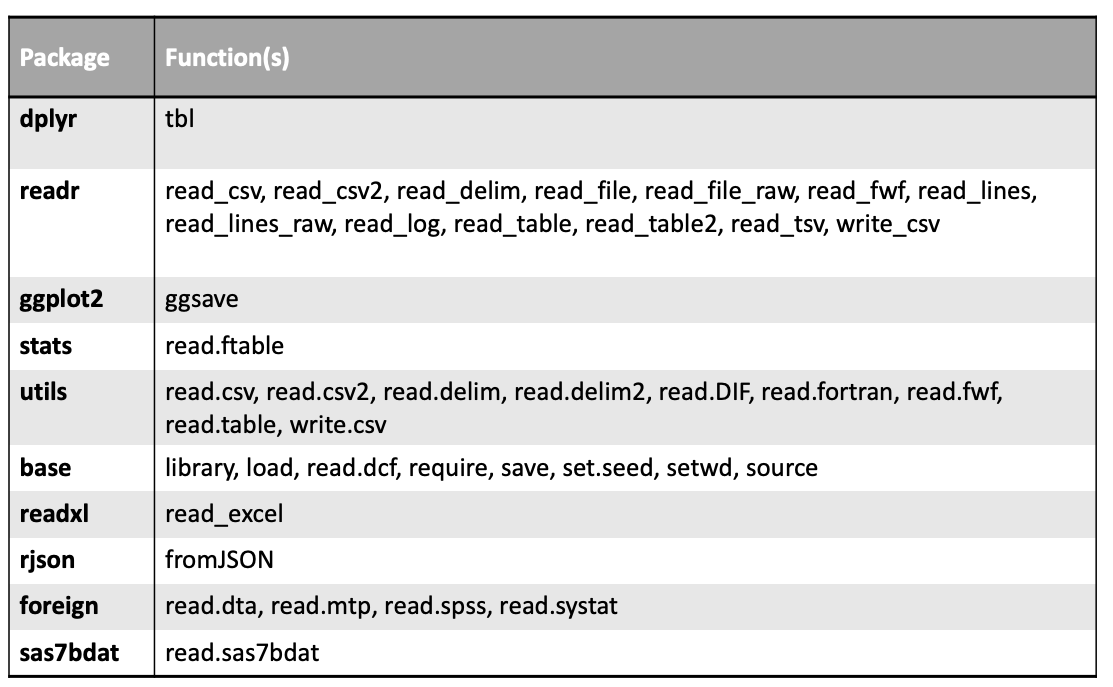
\includegraphics[width=1\linewidth]{figure/shims-list} \caption{List of Functions Shimmed by 'fertile'}\label{fig:unnamed-chunk-34}
\end{figure}
When users perform actions that may threaten reproducibility, the
package's shimmed functions intercept the user's commands and perform
various logging and checking tasks before executing the desired
function.

This allows \texttt{fertile} to warn users when they make mistakes and
also to keep track of past behavior via a log of previously entered
commands.

The process for writing a shim is as follows:
\begin{enumerate}
\def\labelenumi{\arabic{enumi}.}
\item
  Identify an \texttt{R} function that is likely to be involved in
  operations that may break reproducibility. Popular functions
  associated with only one package (e.g., \texttt{read\_csv()} from
  \texttt{readr}) are ideal candidates.
\item
  Create a function in \texttt{fertile} with the same name that takes
  the same arguments (and always the dots \texttt{...}).
\item
  Write this new function so that it:
\end{enumerate}
\begin{enumerate}
\def\labelenumi{\alph{enumi})}
\tightlist
\item
  captures any arguments,
\item
  logs the name of the function called,
\item
  performs any checks on these arguments, and
\item
  calls the original function with the original arguments. Except where
  warranted, the execution looks the same to the user as if they were
  calling the original function.
\end{enumerate}
Most shims, when written, are relatively simple. Several, such as that
for \texttt{library()} are more complex, but many follow the same basic
format that can be seen in this example for\texttt{read\_csv()}:
\begin{Shaded}
\begin{Highlighting}[]
\NormalTok{fertile}\OperatorTok{::}\NormalTok{read_csv}
\end{Highlighting}
\end{Shaded}
\begin{verbatim}
function(file, ...) {
  if (interactive_log_on()) {
    log_push(file, "readr::read_csv")
    check_path_safe(file)
    readr::read_csv(file, ...)
  }
}
<bytecode: 0x7fbd0f3e7658>
<environment: namespace:fertile>
\end{verbatim}
This functionality all occurs without the knowledge of the user.
Consider the example of \texttt{read\_csv()}. \texttt{read\_csv()} is a
very popular function from the \texttt{readr} package for reading in
data files. Users with both \texttt{readr} and \texttt{fertile} loaded,
will experience the following. The user will call \texttt{read\_csv()}
as normal, thinking that they are calling \texttt{readr::read\_csv()}.
However, they will actually be calling \texttt{fertile::read\_csv()}, a
very similar function with the same name. \texttt{fertile::read\_csv()}
will then capture the file path the user provided and check whether it
is reproducible. If it is deemed okay, the function will execute as
intended and read in the data just as \texttt{readr::read\_csv()} would.
If it is deemed non-reproducible, the function will return an error
telling the user to use an alternate file path. Either way,
\texttt{fertile} will record that the user called \texttt{read\_csv()}
and note the path that was provided to it for future reference.

This behavior, however, is dependent \texttt{fertile} remaining at the
top of the \texttt{search()} path so that its functions are called
preferentially over the original functions that it has shimmed. In order
to ensure that the \texttt{fertile} versions of functions (``shims'')
always supersede (``mask'') their original namesakes when called,
\texttt{fertile} uses its own shims of the \texttt{library} and
\texttt{require} functions to manipulate the \texttt{R} \texttt{search}
path so that it is always located in the first position.

In the \texttt{fertile} version of \texttt{library()},\texttt{fertile}
is detached from the search path, the requested package is loaded, and
then \texttt{fertile} is reattached. This ensures that when a user
executes a command, \texttt{R} will check \texttt{fertile} for a
matching function before considering other packages.

\subsection{Hidden Files}\label{hidden-files}

In order to store and analyze information about user behavior and code
structure, \texttt{fertile} utilizes three different types of hidden
files, two of which are \texttt{.csv} format and one of which is a text
file. The hidden \texttt{.csv} files for \texttt{project\_miceps} can be
seen below:
\begin{Shaded}
\begin{Highlighting}[]
\NormalTok{fs}\OperatorTok{::}\KeywordTok{dir_ls}\NormalTok{(}\StringTok{"project_miceps"}\NormalTok{, }\DataTypeTok{all =} \OtherTok{TRUE}\NormalTok{, }\DataTypeTok{glob =} \StringTok{"*_log.csv"}\NormalTok{)}
\end{Highlighting}
\end{Shaded}
\begin{verbatim}
project_miceps/.fertile_log.csv        project_miceps/.fertile_render_log.csv 
\end{verbatim}
The interactive log (\texttt{.fertile\_log.csv}), accessible via
\texttt{log\_report()}, is created as soon as a user executes their
first piece of code that could threaten reproducibility. This file
tracks all of the shimmed functions executed by the user, either in the
console or when running code chunks by hand (rather than knitting a
file). It reports the function called, the relevant argument passed in
(either a file path or \texttt{R} package name), and the time stamp of
when the function was executed. Users can clear the data from this file
and start fresh at any time with \texttt{log\_clear()}.

The render log (\texttt{.fertile\_render\_log.csv}), accessible via
\texttt{render\_log\_report()}, has a similar structure to the
interactive log but is not under the control of the user. It tracks
information about the code contained within \texttt{.R} and
\texttt{.Rmd} files within the project a user is testing for
reproducibility. A new render log file can be generated in one of three
different ways:
\begin{enumerate}
\def\labelenumi{\arabic{enumi}.}
\item
  The first time a user runs one of the major reproducibility checks
  from \texttt{fertile}, such as \texttt{proj\_check()},
  \texttt{proj\_analyze()}, or one of the smaller checks within that
  requires access to the contents of code files.
\item
  Any time a check involving code is called in \texttt{fertile}, the
  package checks to see whether any code files have been updated since
  the last time a render log was generated. If so, a new render log is
  generated.
\item
  The user can generate a new file manually at any time by executing the
  \texttt{proj\_render()} command.
\end{enumerate}
The render log contains information used to run many of the checks in
\texttt{fertile}. It captures the random number generator seed before
and after executing code, notes which packages and files are accessed
and the function with which they were called, and contains a timestamp
of the last time the code was run by \texttt{fertile}. Users cannot
erase it easily.
\begin{Shaded}
\begin{Highlighting}[]
\KeywordTok{render_log_report}\NormalTok{(}\StringTok{"project_miceps"}\NormalTok{)}
\end{Highlighting}
\end{Shaded}
\begin{verbatim}
Reading from /Users/audreybertin/Documents/thesis/index/project_miceps/.fertile_render_log.csv
\end{verbatim}
\begin{verbatim}
# A tibble: 15 x 4
   path                    path_abs                  func    timestamp          
   <chr>                   <chr>                     <chr>   <dttm>             
 1 Seed @ Start            <NA>                      480     2020-10-05 14:16:44
 2 package:dplyr           <NA>                      base::~ 2020-10-05 14:16:44
 3 package:readr           <NA>                      base::~ 2020-10-05 14:16:44
 4 package:tidyr           <NA>                      base::~ 2020-10-05 14:16:44
 5 package:ggplot2         <NA>                      base::~ 2020-10-05 14:16:44
 6 package:purrr           <NA>                      base::~ 2020-10-05 14:16:44
 7 /Users/audreybertin/Do~ /Users/audreybertin/Docu~ readr:~ 2020-10-05 14:16:44
 8 Blot_data_updated.csv   /Users/audreybertin/Docu~ readr:~ 2020-10-05 14:16:44
 9 proteins_v_time.png     /Users/audreybertin/Docu~ ggplot~ 2020-10-05 14:16:45
10 CS_data_redone.csv      /Users/audreybertin/Docu~ readr:~ 2020-10-05 14:16:46
11 citrate_v_time.png      /Users/audreybertin/Docu~ ggplot~ 2020-10-05 14:16:46
12 package:skimr           <NA>                      base::~ 2020-10-05 14:16:47
13 package:stargazer       <NA>                      base::~ 2020-10-05 14:16:48
14 Seed @ End              <NA>                      105     2020-10-05 14:16:49
15 LAST RENDERED           <NA>                      proj_r~ 2020-10-05 14:16:49
\end{verbatim}
These files, integral to many of the functionalities in
\texttt{fertile}, are not visible when looking at the file system. Users
can only access them with functions provided by fertile, and user
permissions are quite restrictive. Except for removing the command
history in the interactive log, users cannot modify their contents, and
neither the render log nor the interactive log can be deleted without
the user modifying their file system. This prevents the files from
mistakenly being tampered with, potentially impairing their
functionality, and ensures that \texttt{fertile} always retains accurate
information of user behavior.

In addition to the two log files, \texttt{fertile} keeps a third hidden
file to track project dependencies. Described in detail in the section
on documentation, this file keeps track of the software setup that a
project is run under. A new version is generated every time
\texttt{fertile} compiles the project code files or when users request
to view the file (via a special access function). Like the log files,
however, there is no simple way to manually modify or delete the file,
ensuring that it does not accidentally get changed in a way that would
damage reproducibility.

\subsection{Environment Variables}\label{environment-variables}

The shims in \texttt{fertile} are designed to be able to write to both
the interactive and render logs. That way, no matter whether a user
calls \texttt{read\_csv()} interactively or writes it in their code
file, \texttt{fertile} will still take note of the fact that the action
has happened.

Given the different purposes of each file, however, it is important that
\texttt{fertile} be able to identify when a function execution should be
saved to the interactive log versus when it should be saved to the
render log.

This information is tracked via a logical environment variable:
\texttt{FERTILE\_RENDER\_MODE}. When \texttt{FERTILE\_RENDER\_MODE} is
\texttt{TRUE}, executed shims are saved to the render log. When it is
\texttt{FALSE}, they are saved to the interactive log.

Since \texttt{fertile} is designed to always be capturing information
about interactive user behavior, \texttt{FERTILE\_RENDER\_MODE} is
\texttt{FALSE} by default.

It is only changed to \texttt{TRUE} when \texttt{fertile} is executing
functions that involve the rendering of \texttt{.R} and \texttt{.Rmd}
code files. At the start of all such functions, \texttt{fertile} sets
the environment variable to \texttt{TRUE}, executes the majority of the
function, and then sets it back to \texttt{FALSE} before exiting. This
ensures that as soon as the function has finished running, all new
commands get executed on the interactive log, rather on the render log
which was just generated.

The example of \texttt{has\_only\_portable\_paths()} illustrates this
functionality. We see several clear steps to this function:
\begin{enumerate}
\def\labelenumi{\arabic{enumi}.}
\item
  The environment variable is set to \texttt{TRUE}, so that
  \texttt{fertile} knows to write any information about shimmed
  functions to the render log.
\item
  If a render log does not yet exist or the project has been updated
  since the last time one was generated, then the project is rendered
  with \texttt{proj\_render()}, generating a new render log.
\item
  This render log is read to find information about the file paths that
  were captured when executing the code files.
\item
  \texttt{fertile} checks to see if the paths are portable and outputs a
  a list of the ones that are not, if any, in addition to some
  information about how to correct that.
\item
  The environment variable is set back to \texttt{FALSE} so that
  interactive behavior is once again captured.
\end{enumerate}
\begin{Shaded}
\begin{Highlighting}[]
\NormalTok{has_only_portable_paths}
\end{Highlighting}
\end{Shaded}
\begin{verbatim}
function(path = ".") {

  Sys.setenv("FERTILE_RENDER_MODE" = TRUE)

  check_is_dir(path)

  if (!has_rendered(path)) {
    proj_render(path)
  }

  paths <- log_report(path) %>%
    dplyr::filter(!grepl("package:", path)) %>%
    dplyr::pull(path)

  good <- paths %>%
    is_path_portable()

  errors <- tibble(
    culprit = as_fs_path(paths[!good]),
    expr = glue("fs::path_rel('{culprit}')")
  )

  Sys.setenv("FERTILE_RENDER_MODE" = FALSE)

  make_check(
    name = "Checking for only portable paths",
    state = all(good),
    problem = "Non-portable paths won't necessarily work for others",
    solution = "Use relative paths.",
    help = "?fs::path_rel",
    errors = errors
  )

}
<bytecode: 0x7fbcf6c28ae0>
<environment: namespace:fertile>
attr(,"req_compilation")
[1] TRUE
\end{verbatim}
\subsection{The Dots (\ldots{})}\label{the-dots}

\texttt{fertile} utilizes the dots (\ldots{}), which allow a function to
accept additional arguments beyond those pre-defined in the function, to
facilitate much of its behavior. The two primary locations the dots are
used are in shims and the \texttt{proj\_check\_some()} function.

Many of the shimmed functions in \texttt{fertile} accept a large number
of arguments. Consider \texttt{read\_csv}. The function requires only
one argument (\texttt{file}) but allows for up to 14.
\begin{Shaded}
\begin{Highlighting}[]
\NormalTok{readr}\OperatorTok{::}\NormalTok{read_csv}
\end{Highlighting}
\end{Shaded}
\begin{verbatim}
function (file, col_names = TRUE, col_types = NULL, locale = default_locale(), 
    na = c("", "NA"), quoted_na = TRUE, quote = "\"", comment = "", 
    trim_ws = TRUE, skip = 0, n_max = Inf, guess_max = min(1000, 
        n_max), progress = show_progress(), skip_empty_rows = TRUE) 
{
    tokenizer <- tokenizer_csv(na = na, quoted_na = quoted_na, 
        quote = quote, comment = comment, trim_ws = trim_ws, 
        skip_empty_rows = skip_empty_rows)
    read_delimited(file, tokenizer, col_names = col_names, col_types = col_types, 
        locale = locale, skip = skip, skip_empty_rows = skip_empty_rows, 
        comment = comment, n_max = n_max, guess_max = guess_max, 
        progress = progress)
}
<bytecode: 0x7fbd0b105120>
<environment: namespace:readr>
\end{verbatim}
When users call the shimmed version of \texttt{read\_csv},
\texttt{fertile} does not need to process any arguments other than
\texttt{file}, since that is the only piece of information directly
relevant to reproducibility. Instead of defining all of the arguments
once again, \texttt{fertile}'s \texttt{read\_csv} is written to accept a
file name and the dots , which then capture and save the additional
input provided by the user. \texttt{fertile} checks the file path, and
then uses the saved dots to then execute \texttt{readr::read\_csv} the
way that the user originally intended.
\begin{Shaded}
\begin{Highlighting}[]
\NormalTok{fertile}\OperatorTok{::}\NormalTok{read_csv}
\end{Highlighting}
\end{Shaded}
\begin{verbatim}
function(file, ...) {
  if (interactive_log_on()) {
    log_push(file, "readr::read_csv")
    check_path_safe(file)
    readr::read_csv(file, ...)
  }
}
<bytecode: 0x7fbd0f3e7658>
<environment: namespace:fertile>
\end{verbatim}
The majority of shims have a similar structure. Since almost all shimmed
functions in \texttt{fertile} take a large number of arguments, the
\texttt{fertile} versions utilize the dots to simplify the process of
capturing this user input and saving it for execution later.

The dots are also utilized in the \texttt{proj\_check\_some} function.
Recall that \texttt{proj\_check\_some} allows users to run a selection
of \texttt{fertile}'s checks by calling a \texttt{tidyselect} helper to
pull out a subset of checks with names matching a certain definition.

This function, which accepts the arguments ``(path,\ldots{}),'' operates
by allowing the users to pass in their \texttt{tidyselect} call to the
dots. The list of available checks are converted into the columns of a
dataframe, then passed through \texttt{dplyr::select(...)}, where the
dots contain the information about the user's \texttt{tidyselect} call.
Then, all of the checks matching the \texttt{tidyselect} call are run on
the provided directory path.

This functionality, along with the other methods of shims, hidden files,
and environment variables, helps improve the user experience of
\texttt{fertile}. These unconventional techniques allow for the reliable
tracking of user behavior behind the scenes and provide functions, like
\texttt{proj\_check\_some}, that are intuitive for the user to operate.

\chapter{\texorpdfstring{Incorporating \texttt{fertile} Into The Greater
Data Science
Community}{Incorporating fertile Into The Greater Data Science Community}}\label{applications}

Finding a solution to addressing reproducibility on a widespread scale
is a challenging problem. Attempts to do so--in academic publishing,
software, and data science education--have made some progress, but many
solutions have significant flaws. Primarily, they either:
\begin{enumerate}
\def\labelenumi{\Alph{enumi})}
\tightlist
\item
  Only address one small aspect of reproducibility--for example,
  software that focuses on version control or a set of journal
  guidelines requesting only that code and data be provided, but giving
  no further detail.
\end{enumerate}
\begin{center}
OR
\end{center}
\begin{enumerate}
\def\labelenumi{\Alph{enumi})}
\setcounter{enumi}{1}
\tightlist
\item
  Are challenging, time consuming, and/or burdensome to implement--for
  example, extensive journal guidelines, complex software packages with
  confusing functions, or academic courses on reproducibility that are
  only accessible to masters' students and take time away from other
  topics.
\end{enumerate}
\texttt{fertile} is an attempt to address reproducibility in a way that
does not fall victim to either of these challenges. Rather than focus on
one area of expertise, \texttt{fertile} contains features focused on
each of the six major components of reproducibility. Its self-contained
nature allows users to address all aspects of reproducibility in one
package; users can achieve near- or complete reproducibility with just a
single piece of software.

\texttt{fertile} also makes the processes of both achieving \emph{and}
checking reproducibility simple and fast. Those looking to check whether
a project is reproducible can almost instantaneously receive a full
report of where the project succeeds and where it fails, and those
looking to improve their reproducibility can receive and act on
\texttt{fertile}'s clear suggestions with minimal effort. Some of the
package's features are enabled automatically and most others can be
accessed with only a handful of functions, all of which are very simple
in function.

Additionally, \texttt{fertile} does not just provide a report on
reproducibility and leave it at that. Instead, it attempts to teach its
users the concepts of reproducibility in the same way that
reproducibility-focused classes are meant to do. Users receive instant
feedback when making mistakes and, when checking work after writing it,
receive reports clearly indicating where issues were found, why they
occurred, and how to correct them.

It is also highly customizable, allowing users to utilize the tool in
the way that fits their needs best. Those who want to focus their
reproducibility checking in a certain direction have that option and
those who want widespread overviews can also have their needs meet.
Users who are interested in going beyond the base functionality of
\texttt{proj\_analyze} and \texttt{proj\_check} also have additional
functions at their disposal that they can use to check reproducibility,
file paths, file types, etc.

\section{\texorpdfstring{Potential Applications of
\texttt{fertile}}{Potential Applications of fertile}}\label{potential-applications-of-fertile}

These features make \texttt{fertile} an excellent tool for addressing
the issue of scientific reproducibility on a widespread scale.
\texttt{fertile} can provide a variety of benefits to users in all
different application domains and with all different experiences. In
this section, we consider the many potential uses of the package.

\subsection{In Journal Review}\label{in-journal-review}

As discussed in Chapter 1, Academic journals have a significant
reproducibility problem. In an attempt to address this, many journals
have instituted reproducibility policies for submitting researchers to
follow. Although a variety of journals have these policies, particularly
in the Statistical and Data Sciences, very few actually go through the
process of verifying that the standards are met. Authors, finding it to
to be a complicated and challenging task, will often not take the
necessary steps to make their work truly reproducible. And journals,
given the amount of time and money required to verify submissions'
reproducibility, will often give submitting authors the benefit of the
doubt in assuming that their work is reproducibile as long as some code
and/or data has been provided. This results in the publishing of many
articles that claim to be reproducible in theory, but do not meet such
standards when tested in practice.

\texttt{fertile} could provide significant assistance with this process.
Journals could integrate \texttt{fertile} into their article review
workflow, running the primary checks in the package to see whether they
are passed or if they fail. This would be an incredibly fast process: as
long as a journal required that all submissions in \texttt{R} be in the
\texttt{R\ Project} format, one reviewer could load the submission, run
\texttt{fertile}, and receive a summary of the submission's
reproducibility in a matter of minutes.

Journals could easily build a standard of reproducibility around
\texttt{fertile}'s checking system, requiring that a minimum set of
checks be passed for any submitted article to be approved. This would
improve the quality of submitted work and reduce the burden on journals
of ensuring reproducibility in their published articles. Since
\texttt{fertile} is publicly available, users would have access to the
exact same testing system as any journal and therefore be able to ensure
before submission that their articles would meet the provided standards.

This process would be much faster than that employed currently at the
American Journal of Political Science, which goes through a thorough,
multi-week-long reproducibility confirmation procedure for all submitted
articles. Submitting researchers would know exactly which goals they
were trying to achieve. They could download \texttt{fertile} on their
own, run it on their project, check to see if their goals are met, and
take the recommended steps to address failures if not. Then, upon
submission, the journal would only need to run \texttt{fertile}'s
functions once to confirm that the standards were met.

Although this would only address a small aspect of reproducibility--that
involving data analysis projects written in R--it would provide a
significant time- and money-saving impact for both authors and reviewers
in that domain.

\subsection{For Teaching
Reproducibility}\label{for-teaching-reproducibility}

\texttt{fertile} could also be integrated into Statistical and Data
Sciences coursework in order to educate students on topics of
reproducibility.

Many of the existing programs to teach reproducibility are courses
focused on replication studies, where students must take a published
paper and replicate the steps within completely. This process, which
includes requesting the necessary data and code files from the original
author(s) and sometimes even expanding the existing analysis further,
often requires that participants have knowledge of data analysis and the
scientific research process to be successful. As a result, such courses
focused on reproducibility tend to exist only at the graduate level.

Undergraduate students, therefore, do not get exposed to reproducibility
very often. There are a few exceptions--for instance, introductory
courses at Smith College and Duke University that integrate RMarkdown to
promote reproducible workflows--but overall, reproducibility is not
covered in data science courses the undergraduate level.

\texttt{fertile} could help change this, allowing for many more colleges
and universities to integrate reproducibility into their courses. The
barriers to entry for using and benefitting from the package are very
low, requiring only that participating students have:
\begin{itemize}
\tightlist
\item
  R and RStudio installed on their computer
\item
  Knowledge of how to install a package from GitHub and load it into
  their environment
\item
  Knowledge of how to create an R project
\item
  Knowledge of how to run basic functions and input simple file paths
\end{itemize}
Though the process may entail some confusion and troubleshooting at
first, even those brand new to \texttt{R} could succeed in overcoming
these barriers in only a few days of class. As a result,
\texttt{fertile} could provide professors with an opportunity to teach
reproducibility concepts in introductory level courses.

\texttt{fertile} could easily integrate into coursework in a similar way
to how RMarkdown was integrated at Smith College and Duke University.
While there is not only one way to utilize the software in class, a
potential use of \texttt{fertile} could look as follows:

At the beginning of their courses, the professor provides their students
with a brief introduction to reproducibility, including its importance
and a basic description of how it is achieved. Shortly after, they
introduce R Projects and the \texttt{fertile} package, explaining that
they are tools to help with reproducibility. Then, they institute a
requirement for all submitted homework assignments in the course:
students must create and submit their work in the R Project format, but
prior to submission must run \texttt{fertile} on their project to ensure
that it passes reproducibility standards. When reproducibility errors
inevitably occur, they can be used as teaching moments: the professor
can share the error, explain why it happened, walk through
\texttt{fertile}'s response to it, and interactively work with students
to illustrate how it can be fixed.

The integration of \texttt{fertile} in this way would be an excellent
method to introduce students to reproducibility concepts early on in
their data science education, but at a low cost to the professor.

Students would learn about reproducibility at the beginning of their
data science education, which provides a variety of benefits over being
introduced later on--in graduate school or through independent research
on the topic:
\begin{itemize}
\item
  Teaching reproducibility early on gives students important research
  tools and understanding before they conduct any of their own important
  analysis.
\item
  Practicing before students are believed to be skilled and highly
  educated in data science gives them an opportunity to fail and learn
  without fear of judgement.
\item
  Integrating concepts early helps ingrain them in the minds of
  students, ensuring that reproducibility begins to come naturally to
  them.
\end{itemize}
These students would then be prepared for entering the research world
and contributing to data science work in a transparent and reproducible
way.

** INTRODUCE EXPERIMENT HERE **

\texttt{fertile} is designed to: 1) be simple enough that users with
minimal \texttt{R} experience can use the package without issue, 2)
increase the reproducibility of work produced by its users, and 3)
educate its users on why their work is or is not reproducible and
provide guidance on how to address any problems.

To test \texttt{fertile}'s effectiveness, we began an initial randomized
control trial of the package on an introductory undergraduate data
science course at Smith College in Spring 2020 \textbf{ADD FOOTNOTE}
(This study was approved by Smith College IRB, Protocol \#19-032).

The experiment was structured as follows:

1.Students are given a form at the start of the semester asking whether
they consent to participate in a study on data science education. In
order to successfully consent, they must provide their system username,
collected through the command \texttt{Sys.getenv("LOGNAME")}. To
maintain privacy the results are then transformed into a hexadecimal
string via the \texttt{md5()} hashing function.
\begin{enumerate}
\def\labelenumi{\arabic{enumi}.}
\setcounter{enumi}{1}
\item
  These hexadecimal strings are then randomly assigned into equally
  sized groups, one experimental group that receives the features of
  \texttt{fertile} and one group that receives a control.
\item
  The students are then asked to download a package called
  \texttt{sds192} (the course number and prefix), which was created for
  the purpose of this trial. It leverages an \texttt{.onAttach()}
  function to scan the \texttt{R} environment and collect the username
  of the user who is loading the package and run it through the same
  hashing algorithm as used previously. It then identifies whether that
  user belongs to the experimental or the control group. Depending on
  the group they are in, they receive a different version of the
  package.
\item
  The experimental group receives the basic \texttt{sds192} package,
  which consists of some data sets and \texttt{R} Markdown templates
  necessary for completing homework assignments and projects in the
  class, but also has \texttt{fertile} installed and loaded silently in
  the background. The package's proactive features are enabled, and
  therefore users will receive warning messages when they use absolute
  or non-portable paths or attempt to change their working directory.
  The control group receives only the basic \texttt{sds192} package,
  including its data sets and \texttt{R} Markdown templates. All
  students from both groups then use their version of the package
  throughout the semester on a variety of projects.
\item
  Both groups are given a short quiz on different components of
  reproducibility that are intended to be taught by \texttt{fertile} at
  both the beginning and end of the semester. Their scores are then
  compared to see whether one group learned more than the other group or
  whether their scores were essentially equivalent. Additionally, for
  every homework assignment submitted, the professor takes note of
  whether or not the project compiles successfully.
\end{enumerate}
Based on the results, we hope to determine whether \texttt{fertile} was
successful at achieving its intended goals. A lack of notable difference
between the \emph{experimental} and \emph{control} groups in terms of
the number of code-related questions asked throughout the semester would
indicate that \texttt{fertile} achieved its goal of simplicity. A higher
average for the \emph{experimental} group in terms of the number of
homework assignments that compiled successfully would indicate that
\texttt{fertile} was successful in increasing reproducibility. A greater
increase over the semester in the reproducibility quiz scores for
students in the \emph{experimental} group compared with the
\emph{control} group would indicate that \texttt{fertile} achieved its
goal of educating users on reproducibility. Success according to these
metrics would provide evidence showing \texttt{fertile}'s benefit as
tool to help educators introduce reproducibility concepts in the
classroom.

\subsection{In Other Areas}\label{in-other-areas}

\texttt{fertile} can also provide benefits in other domains. Though not
an exhausted list, some of the potential uses of the software are:
\begin{itemize}
\item
  \emph{Private Companies}: Data analysis-focused companies could
  require their employees to use \texttt{fertile} to check the
  reproducibility of their projects before presenting them to clients.
  This would help such companies ensure that clients could trust the
  results that were being produced.
\item
  \emph{Conferences}: Similar to academic journals, conferences
  promoting open research could require that papers written in
  \texttt{R} pass a \texttt{fertile} check as a condition for
  acceptance. Even if there were an exception given for those using
  confidential/identifiable data, this would likely increase the overall
  reproducibility of conference papers significantly.
\item
  \emph{Informal Data Analysis}: A lot of content in the \texttt{R}
  community is created purely for fun and interest. Outside of work,
  many \texttt{R} users will create data visualizations or analyses for
  their own private blogs or their twitter. Sometimes, users will also
  participate in community events like Tidy Tuesday, a weekly social
  project where a data set is posted and users are asked to analyze it
  and create a visualization of their choice. Many people use these
  informal analyses as an opportunity for learning and discussion, often
  sharing them on social media to try and get feedback on their work.
  Ensuring that the work is reproducible would facilitate this process.
  Users could run their project files through \texttt{fertile} to check
  that they are reproducible and post a link to download them. This
  would then allow others to run the code on their own to understand how
  it works and more easily be able to make suggestions as to how to
  improve it!
\end{itemize}
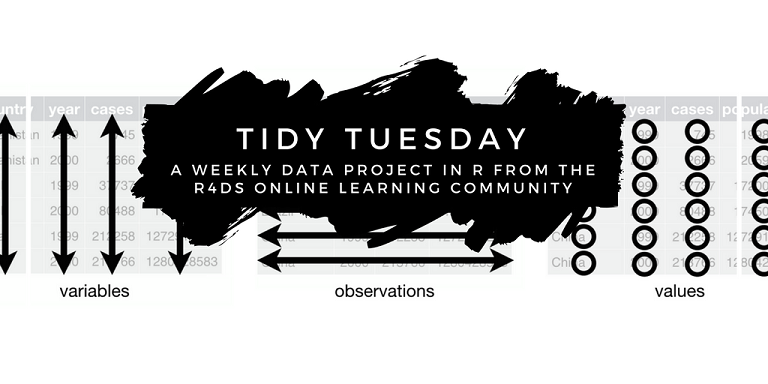
\includegraphics[width=1\linewidth]{figure/tidytuesday}

\texttt{fertile} is incredibly versatile in its applicability. It can be
used anywhere from informal data analysis projects to academic journal
review.

\chapter*{Conclusion}\label{conclusion}
\addcontentsline{toc}{chapter}{Conclusion}

\texttt{fertile} is an \texttt{R} package that lowers barriers to
reproducible data analysis projects in \texttt{R}, providing a wide
array of checks and suggestions addressing many different aspects of
project reproducibility, including file organization, file path usage,
documentation, and dependencies. \texttt{fertile} is meant to be
educational, providing informative error messages that indicate why
users' mistakes are problematic and sharing recommendations on how to
fix them. The package is designed in this way so as to promote a greater
understanding of reproducibility concepts in its users, with the goal of
increasing the overall awareness and understanding of reproducibility in
the \texttt{R} community.

The package has very low barriers to entry, making it accessible to
users with various levels of background knowledge. Unlike many other
\texttt{R} packages focused on reproducibility that are currently
available, the features of \texttt{fertile} can be accessed almost
effortlessly. Many of the retroactive features can be accessed in only
two lines of code requiring minimal arguments and some of the proactive
features can be accessed with no additional effort beyond loading the
package. This, in combination with the fact that \texttt{fertile} does
not focus on one specific area of reproducibility, instead covering
(albeit in less detail) a wide variety of topics, means that
\texttt{fertile} makes it easy for data analysts of all skill levels to
quickly gain a better understanding of the reproducibility of the work.

In the moment, it often feels easiest to take a shortcut---to use an
absolute path or change a working directory. However, when considering
the long term path of a project, spending the extra time to improve
reproducibility is worthwhile. \texttt{fertile}'s user-friendly features
can help data analysts avoid these harmful shortcuts with minimal
effort.

\appendix

\chapter{The First Appendix}\label{the-first-appendix}

This first appendix includes all of the R chunks of code that were
hidden throughout the document (using the \texttt{include\ =\ FALSE}
chunk tag) to help with readibility and/or setup.

\textbf{In the main Rmd file}
\begin{Shaded}
\begin{Highlighting}[]
\CommentTok{# This chunk ensures that the thesisdown package is}
\CommentTok{# installed and loaded. This thesisdown package includes}
\CommentTok{# the template files for the thesis.}
\ControlFlowTok{if}\NormalTok{ (}\OperatorTok{!}\KeywordTok{require}\NormalTok{(remotes)) \{}
  \ControlFlowTok{if}\NormalTok{ (params}\OperatorTok{$}\StringTok{`}\DataTypeTok{Install needed packages for \{thesisdown\}}\StringTok{`}\NormalTok{) \{}
    \KeywordTok{install.packages}\NormalTok{(}\StringTok{"remotes"}\NormalTok{, }\DataTypeTok{repos =} \StringTok{"https://cran.rstudio.com"}\NormalTok{)}
\NormalTok{  \} }\ControlFlowTok{else}\NormalTok{ \{}
    \KeywordTok{stop}\NormalTok{(}
      \KeywordTok{paste}\NormalTok{(}\StringTok{'You need to run install.packages("remotes")",}
\StringTok{            "first in the Console.'}\NormalTok{)}
\NormalTok{    )}
\NormalTok{  \}}
\NormalTok{\}}
\ControlFlowTok{if}\NormalTok{ (}\OperatorTok{!}\KeywordTok{require}\NormalTok{(thesisdown)) \{}
  \ControlFlowTok{if}\NormalTok{ (params}\OperatorTok{$}\StringTok{`}\DataTypeTok{Install needed packages for \{thesisdown\}}\StringTok{`}\NormalTok{) \{}
\NormalTok{    remotes}\OperatorTok{::}\KeywordTok{install_github}\NormalTok{(}\StringTok{"ismayc/thesisdown"}\NormalTok{)}
\NormalTok{  \} }\ControlFlowTok{else}\NormalTok{ \{}
    \KeywordTok{stop}\NormalTok{(}
      \KeywordTok{paste}\NormalTok{(}
        \StringTok{"You need to run"}\NormalTok{,}
        \StringTok{'remotes::install_github("ismayc/thesisdown")'}\NormalTok{,}
        \StringTok{"first in the Console."}
\NormalTok{      )}
\NormalTok{    )}
\NormalTok{  \}}
\NormalTok{\}}
\KeywordTok{library}\NormalTok{(thesisdown)}
\CommentTok{# Set how wide the R output will go}
\end{Highlighting}
\end{Shaded}
\chapter{The Second Appendix, for
Fun}\label{the-second-appendix-for-fun}

\backmatter

\chapter*{References}\label{references}
\addcontentsline{toc}{chapter}{References}

\markboth{References}{References}

\noindent

\setlength{\parindent}{-0.20in} \setlength{\leftskip}{0.20in}
\setlength{\parskip}{8pt}

\hypertarget{refs}{}
\hypertarget{ref-aee-policy}{}
American Economic Association. (2020). Data and code availability
policy. Retrieved from
\url{https://www.aeaweb.org/journals/data/data-code-policy}

\hypertarget{ref-ajps-guidelines}{}
American Journal of Political Science. (2016, May). Guidelines for
preparing replication files. Retrieved from
\url{https://ajps.org/wp-content/uploads/2018/05/ajps_replication-guidelines-2-1.pdf}

\hypertarget{ref-asa-guide}{}
American Statistical Association. (2020). JASA acs reproducibility
guide. Retrieved from
\url{https://jasa-acs.github.io/repro-guide/pages/author-guidelines}

\hypertarget{ref-nature-psych}{}
Baker, M. (2015). Over half of psychological studies fail
reproducibility test. \emph{Nature}. Retrieved from
\url{https://www.nature.com/news/over-half-of-psychology-studies-fail-reproducibility-test-1.18248}

\hypertarget{ref-nature-crisis}{}
Baker, M. (2016). 1,500 scientists lift the lid on reproducibility.
\emph{Nature}. Retrieved from
\url{https://www.nature.com/news/1-500-scientists-lift-the-lid-on-reproducibility-1.19970}

\hypertarget{ref-baumer2014r}{}
Baumer, B., Cetinkaya-Rundel, M., Bray, A., Loi, L., \& Horton, N. J.
(2014). R markdown: Integrating a reproducible analysis tool into
introductory statistics. \emph{arXiv Preprint arXiv:1402.1894}.

\hypertarget{ref-begley2012raise}{}
Begley, C. G., \& Ellis, L. M. (2012). Raise standards for preclinical
cancer research. \emph{Nature}, \emph{483}(7391), 531--533.

\hypertarget{ref-R-workflowr}{}
Blischak, J., Carbonetto, P., \& Stephens, M. (2019). Workflowr: A
framework for reproducible and collaborative data science. Retrieved
from \url{https://CRAN.R-project.org/package=workflowr}

\hypertarget{ref-arlington}{}
Bollen, K., Cacioppo, J. T., Kaplan, R. M., Krosnick, J. A., Olds, J.
L., \& Dean, H. (2015). Report of the subcommittee on replicability in
science advisory committee to the nsf sbe directorate. Retrieved from
\url{https://www.nsf.gov/sbe/SBE_Spring_2015_AC_Meeting_Presentations/Bollen_Report_on_Replicability_SubcommitteeMay_2015.pdf}

\hypertarget{ref-broman}{}
Broman, K. (2019). Initial steps toward reproducible research: Organize
your data and code. \emph{Sitewide ATOM}. Retrieved from
\url{https://kbroman.org/steps2rr/pages/organize.html}

\hypertarget{ref-exp-results}{}
Cambridge University Press. (2020). Experimental results - transparency
and openness policy. Retrieved from
\url{https://www.cambridge.org/core/journals/experimental-results/information/transparency-and-openness-policy}

\hypertarget{ref-claerbout}{}
Claerbout, J. F., \& Karrenbach, M. (1992). Electronic documents give
reproducible research a new meaning. In \emph{SEG technical program
expanded abstracts 1992} (pp. 601--604). Society of Exploration
Geophysicists.

\hypertarget{ref-cooper2017guide}{}
Cooper, N., Hsing, P.-Y., Croucher, M., Graham, L., James, T.,
Krystalli, A., \& Michonneau, F. (2017). A guide to reproducible code in
ecology and evolution. \emph{British Ecological Society}. Retrieved from
\url{https://www.britishecologicalsociety.org/wp-content/uploads/2017/12/guide-to-reproducible-code.pdf}

\hypertarget{ref-eisner-reproducibility}{}
Eisner, D. A. (2018). Reproducibility of science: Fraud, impact factors
and carelessness. \emph{Journal of Molecular and Cellular Cardiology},
\emph{114}, 364--368.
\url{http://doi.org/https://doi.org/10.1016/j.yjmcc.2017.10.009}

\hypertarget{ref-epstein2002immediate}{}
Epstein, M. L., Lazarus, A. D., Calvano, T. B., Matthews, K. A., Hendel,
R. A., Epstein, B. B., \& Brosvic, G. M. (2002). Immediate feedback
assessment technique promotes learning and corrects inaccurate first
responses. \emph{The Psychological Record}, \emph{52}(2), 187--201.

\hypertarget{ref-sep-scientific-reproducibility}{}
Fidler, F., \& Wilcox, J. (2018). Reproducibility of scientific results.
In E. N. Zalta (Ed.), \emph{The stanford encyclopedia of philosophy}
(Winter 2018).
\url{https://plato.stanford.edu/archives/win2018/entries/scientific-reproducibility/};
Metaphysics Research Lab, Stanford University.

\hypertarget{ref-R-orderly}{}
FitzJohn, R., Ashton, R., Hill, A., Eden, M., Hinsley, W., Russell, E.,
\& Thompson, J. (2020). Orderly: Lightweight reproducible reporting.
Retrieved from \url{https://CRAN.R-project.org/package=orderly}

\hypertarget{ref-unix}{}
Gancarz, M. (2003). \emph{Linux and the unix philosophy} (2nd ed.).
Woburn, MA: Digital Press.

\hypertarget{ref-Goodman341ps12}{}
Goodman, S. N., Fanelli, D., \& Ioannidis, J. P. A. (2016). What does
research reproducibility mean? \emph{Science Translational Medicine},
\emph{8}(341), 1--6. \url{http://doi.org/10.1126/scitranslmed.aaf5027}

\hypertarget{ref-bioessays-gosselin}{}
Gosselin, R.-D. (2020). Statistical analysis must improve to address the
reproducibility crisis: The access to transparent statistics (acts) call
to action. \emph{BioEssays}, \emph{42}(1), 1900189.
\url{http://doi.org/10.1002/bies.201900189}

\hypertarget{ref-hardwicke2018data}{}
Hardwicke, T. E., Mathur, M. B., MacDonald, K., Nilsonne, G., Banks, G.
C., Kidwell, M. C., \ldots{} others. (2018). Data availability,
reusability, and analytic reproducibility: Evaluating the impact of a
mandatory open data policy at the journal cognition. \emph{Royal Society
Open Science}, \emph{5}(8), 180448. Retrieved from
\url{https://royalsocietypublishing.org/doi/full/10.1098/rsos.180448}

\hypertarget{ref-R-tidyselect}{}
Henry, L., \& Wickham, H. (2020). Tidyselect: Select from a set of
strings. Retrieved from
\url{https://CRAN.R-project.org/package=tidyselect}

\hypertarget{ref-hermans2017programming}{}
Hermans, F., \& Aldewereld, M. (2017). Programming is writing is
programming. In \emph{Companion to the first international conference on
the art, science and engineering of programming} (pp. 1--8).

\hypertarget{ref-berkeley_teaching}{}
Hillenbrand, S. (2014). Reproducible and collaborative: Teaching the
data science life. Berkeley Science Review. Retrieved from
\url{https://berkeleysciencereview.com/2014/06/reproducible-collaborative-data-science/}

\hypertarget{ref-horton2014teaching}{}
Horton, N. J., Baumer, B. S., \& Wickham, H. (2014). Teaching precursors
to data science in introductory and second courses in statistics.
\emph{arXiv Preprint arXiv:1401.3269}.

\hypertarget{ref-hrynaszkiewicz2020publishers}{}
Hrynaszkiewicz, I. (2020). Publishers' responsibilities in promoting
data quality and reproducibility. \emph{Handbook of Experimental
Pharmacology}, \emph{257}, 319--348.
\url{http://doi.org/https://doi.org/10.1007/164_2019_290}

\hypertarget{ref-higher-ed}{}
Jacoby, W. G., Lafferty-Hess, S., \& Christian, T.-M. (2017). Should
journals be responsible for reproducibility? Inside Higher Ed. Retrieved
from
\url{https://www.insidehighered.com/blogs/rethinking-research/should-journals-be-responsible-reproducibility}

\hypertarget{ref-janz2016bringing}{}
Janz, N. (2016). Bringing the gold standard into the classroom:
Replication in university teaching. \emph{International Studies
Perspectives}, \emph{17}(4), 392--407.

\hypertarget{ref-jcgs-guide}{}
Journal of Computational and Graphical Statistics. (2020). Instructions
for authors. Retrieved from
\url{https://www.tandfonline.com/action/authorSubmission?show=instructions\&journalCode=ucgs20}

\hypertarget{ref-jss-guide}{}
Journal of Statistical Software. (2020). Instructions for authors.
Retrieved from
\url{https://www.jstatsoft.org/pages/view/authors\#review-process.}

\hypertarget{ref-kitzes2017practice}{}
Kitzes, J., Turek, D., \& Deniz, F. (2017). \emph{The practice of
reproducible research: Case studies and lessons from the data-intensive
sciences}. Berkeley, CA: University of California Press. Retrieved from
\url{https://www.practicereproducibleresearch.org}

\hypertarget{ref-leopold2015increased}{}
Leopold, S. S. (2015). Editorial: Increased manuscript submissions
prompt journals to make hard choices. \emph{Clinical Orthopaedics and
Related Research}, \emph{473}(3), 753--755.
\url{http://doi.org/10.1007/s11999-014-4129-1}

\hypertarget{ref-lupia2014openness}{}
Lupia, A., \& Elman, C. (2014). Openness in political science: Data
access and research transparency. \emph{PS, Political Science \&
Politics}, \emph{47}(1), 19.

\hypertarget{ref-r-opensci}{}
Martinez, C., Hollister, J., Marwick, B., Szöcs, E., Zeitlin, S.,
Kinoshita, B. P., \ldots{} Meinke, B. (2018). Reproducibility in
Science: A Guide to enhancing reproducibility in scientific results and
writing. Retrieved from
\url{http://ropensci.github.io/reproducibility-guide/}

\hypertarget{ref-R-rrtools}{}
Marwick, B. (2019). Rrtools: Creates a reproducible research compendium.
Retrieved from \url{https://github.com/benmarwick/rrtools}

\hypertarget{ref-marwick2018packaging}{}
Marwick, B., Boettiger, C., \& Mullen, L. (2018). Packaging data
analytical work reproducibly using R (and friends). \emph{The American
Statistician}, \emph{72}(1), 80--88.
\url{http://doi.org/doi.org/10.1080/00031305.2017.1375986}

\hypertarget{ref-engineering-reproducibility}{}
McArthur, S. L. (2019). Repeatability, reproducibility, and
replicability: Tackling the 3R challenge in biointerface science and
engineering. \emph{Biointerphases}, \emph{14}(2), 1--2.
\url{http://doi.org/10.1116/1.5093621}

\hypertarget{ref-R-reproducible}{}
McIntire, E. J. B., \& Chubaty, A. M. (2020). Reproducible: A set of
tools that enhance reproducibility beyond package management. Retrieved
from \url{https://CRAN.R-project.org/package=reproducible}

\hypertarget{ref-bio-principles}{}
National Institutes of Health. (2014, June). Principles and guidelines
for reporting preclinical research. Retrieved from
\url{https://www.nih.gov/research-training/rigor-reproducibility/principles-guidelines-reporting-preclinical-research}

\hypertarget{ref-R-drake}{}
OpenSci, R. (2020). Drake: A pipeline toolkit for reproducible
computation at scale. Retrieved from
\url{https://cran.r-project.org/package=drake}

\hypertarget{ref-wercker}{}
Oracle Corporation. (2019). Wercker. Retrieved from
\url{https://github.com/wercker/wercker}

\hypertarget{ref-r-journal}{}
R Journal Editors. (2020). Instructions for authors. Retrieved from
\url{https://journal.r-project.org/share/author-guide.pdf}

\hypertarget{ref-coreteam-extensions}{}
R-Core-Team. (2020). Writing r extensions. \emph{R Foundation for
Statistical Computing}. Retrieved from
\url{http://cran.stat.unipd.it/doc/manuals/r-release/R-exts.pdf}

\hypertarget{ref-R-checkers}{}
Ross, N., DeCicco, L., \& Randhawa, N. (2018). Checkers: Automated
checking of best practices for research compendia. Retrieved from
\url{https://github.com/ropenscilabs/checkers/blob/master/DESCRIPTIONr}

\hypertarget{ref-policy-effectiveness}{}
Stodden, V., Seiler, J., \& Ma, Z. (2018a). An empirical analysis of
journal policy effectiveness for computational reproducibility.
\emph{Proceedings of the National Academy of Sciences}, \emph{115}(11),
2584--2589. Retrieved from
\url{https://www.pnas.org/content/115/11/2584}

\hypertarget{ref-Stodden2584}{}
Stodden, V., Seiler, J., \& Ma, Z. (2018b). An empirical analysis of
journal policy effectiveness for computational reproducibility.
\emph{Proceedings of the National Academy of Sciences}, \emph{115}(11),
2584--2589. \url{http://doi.org/10.1073/pnas.1708290115}

\hypertarget{ref-ams-guide}{}
The American Statistician. (2020). Instructions for authors. Retrieved
from
\url{https://www.tandfonline.com/action/authorSubmission?show=instructions\&journalCode=utas20}

\hypertarget{ref-R-renv}{}
Ushey, K., \& RStudio. (2020). Renv: Project environments. Retrieved
from \url{https://cran.r-project.org/web/packages/renv/index.html}

\hypertarget{ref-plos-biology}{}
Wallach, J. D., Boyack, K. W., \& Ioannidis, J. P. A. (2018).
Reproducible research practices, transparency, and open access data in
the biomedical literature, 2015-2017. \emph{PLOS Biology},
\emph{16}(11), 1--20. \url{http://doi.org/10.1371/journal.pbio.2006930}

\hypertarget{ref-hadley-packages}{}
Wickham, H. (2015). \emph{R packages} (1st ed.). Sebastopol, CA:
O'Reilly Media, Inc.

\hypertarget{ref-top-guidelines}{}
Woolston, C. (2020). TOP factor rates journals on transparency,
openness. Nature Index. Retrieved from
\url{https://www.natureindex.com/news-blog/top-factor-rates-journals-on-transparency-openness}

\hypertarget{ref-yu2019toward}{}
Yu, B., \& Hu, X. (2019). Toward training and assessing reproducible
data analysis in data science education. \emph{Data Intelligence},
\emph{1}(4), 381--392.


% Index?

\end{document}
